% Options for packages loaded elsewhere
\PassOptionsToPackage{unicode}{hyperref}
\PassOptionsToPackage{hyphens}{url}
%
\documentclass[
]{article}
\usepackage[nobottomtitles]{titlesec}
\usepackage{rotating}
\title{A Living Review on the Usability of Interactive Theorem Provers}
\author{Sam Nolan}
\date{28 October 2021}

\usepackage{amsmath,amssymb}
\usepackage{lmodern}
\usepackage{iftex}
\ifPDFTeX
  \usepackage[T1]{fontenc}
  \usepackage[utf8]{inputenc}
  \usepackage{textcomp} % provide euro and other symbols
\else % if luatex or xetex
  \usepackage{unicode-math}
  \defaultfontfeatures{Scale=MatchLowercase}
  \defaultfontfeatures[\rmfamily]{Ligatures=TeX,Scale=1}
\fi
% Use upquote if available, for straight quotes in verbatim environments
\IfFileExists{upquote.sty}{\usepackage{upquote}}{}
\IfFileExists{microtype.sty}{% use microtype if available
  \usepackage[]{microtype}
  \UseMicrotypeSet[protrusion]{basicmath} % disable protrusion for tt fonts
}{}
\makeatletter
\@ifundefined{KOMAClassName}{% if non-KOMA class
  \IfFileExists{parskip.sty}{%
    \usepackage{parskip}
  }{% else
    \setlength{\parindent}{0pt}
    \setlength{\parskip}{6pt plus 2pt minus 1pt}}
}{% if KOMA class
  \KOMAoptions{parskip=half}}
\makeatother
\usepackage{xcolor}
\IfFileExists{xurl.sty}{\usepackage{xurl}}{} % add URL line breaks if available
\IfFileExists{bookmark.sty}{\usepackage{bookmark}}{\usepackage{hyperref}}
\hypersetup{
  pdftitle={A Living Review on the Usability of Interactive Theorem Provers},
  pdfauthor={Sam Nolan},
  hidelinks,
  pdfcreator={LaTeX via pandoc}}
\urlstyle{same} % disable monospaced font for URLs
\usepackage{geometry}
\geometry{a4paper, portrait, margin=3cm}
\usepackage{listings}
\newcommand{\passthrough}[1]{#1}
\lstset{defaultdialect=[5.3]Lua}
\lstset{defaultdialect=[x86masm]Assembler}
\usepackage{longtable,booktabs,array}
\usepackage{calc} % for calculating minipage widths
% Correct order of tables after \paragraph or \subparagraph
\usepackage{etoolbox}
\makeatletter
\patchcmd\longtable{\par}{\if@noskipsec\mbox{}\fi\par}{}{}
\makeatother
% Allow footnotes in longtable head/foot
\IfFileExists{footnotehyper.sty}{\usepackage{footnotehyper}}{\usepackage{footnote}}
\makesavenoteenv{longtable}
\usepackage{graphicx}
\makeatletter
\def\maxwidth{\ifdim\Gin@nat@width>\linewidth\linewidth\else\Gin@nat@width\fi}
\def\maxheight{\ifdim\Gin@nat@height>\textheight\textheight\else\Gin@nat@height\fi}
\makeatother
% Scale images if necessary, so that they will not overflow the page
% margins by default, and it is still possible to overwrite the defaults
% using explicit options in \includegraphics[width, height, ...]{}
\setkeys{Gin}{width=\maxwidth,height=\maxheight,keepaspectratio}
% Set default figure placement to htbp
\makeatletter
\def\fps@figure{htbp}
\makeatother
\setlength{\emergencystretch}{3em} % prevent overfull lines
\providecommand{\tightlist}{%
  \setlength{\itemsep}{0pt}\setlength{\parskip}{0pt}}
\setcounter{secnumdepth}{5}
\newlength{\cslhangindent}
\setlength{\cslhangindent}{1.5em}
\newlength{\csllabelwidth}
\setlength{\csllabelwidth}{3em}
\newlength{\cslentryspacingunit} % times entry-spacing
\setlength{\cslentryspacingunit}{\parskip}
\newenvironment{CSLReferences}[2] % #1 hanging-ident, #2 entry spacing
 {% don't indent paragraphs
  \setlength{\parindent}{0pt}
  % turn on hanging indent if param 1 is 1
  \ifodd #1
  \let\oldpar\par
  \def\par{\hangindent=\cslhangindent\oldpar}
  \fi
  % set entry spacing
  \setlength{\parskip}{#2\cslentryspacingunit}
 }%
 {}
\usepackage{calc}
\newcommand{\CSLBlock}[1]{#1\hfill\break}
\newcommand{\CSLLeftMargin}[1]{\parbox[t]{\csllabelwidth}{#1}}
\newcommand{\CSLRightInline}[1]{\parbox[t]{\linewidth - \csllabelwidth}{#1}\break}
\newcommand{\CSLIndent}[1]{\hspace{\cslhangindent}#1}

\makeatletter
\@ifpackageloaded{subfig}{}{\usepackage{subfig}}
\@ifpackageloaded{caption}{}{\usepackage{caption}}
\captionsetup[subfloat]{margin=0.5em}
\AtBeginDocument{%
\renewcommand*\figurename{Figure}
\renewcommand*\tablename{Table}
}
\AtBeginDocument{%
\renewcommand*\listfigurename{List of Figures}
\renewcommand*\listtablename{List of Tables}
}
\newcounter{pandoccrossref@subfigures@footnote@counter}
\newenvironment{pandoccrossrefsubfigures}{%
\setcounter{pandoccrossref@subfigures@footnote@counter}{0}
\begin{figure}\centering%
\gdef\global@pandoccrossref@subfigures@footnotes{}%
\DeclareRobustCommand{\footnote}[1]{\footnotemark%
\stepcounter{pandoccrossref@subfigures@footnote@counter}%
\ifx\global@pandoccrossref@subfigures@footnotes\empty%
\gdef\global@pandoccrossref@subfigures@footnotes{{##1}}%
\else%
\g@addto@macro\global@pandoccrossref@subfigures@footnotes{, {##1}}%
\fi}}%
{\end{figure}%
\addtocounter{footnote}{-\value{pandoccrossref@subfigures@footnote@counter}}
\@for\f:=\global@pandoccrossref@subfigures@footnotes\do{\stepcounter{footnote}\footnotetext{\f}}%
\gdef\global@pandoccrossref@subfigures@footnotes{}}
\newcommand*\listoflistings\lstlistoflistings
\AtBeginDocument{%
\renewcommand*{\lstlistlistingname}{List of Listings}
}
\makeatother
\ifLuaTeX
  \usepackage{selnolig}  % disable illegal ligatures
\fi
\definecolor{verb_border}{rgb}{0.7,0.7,1}
\definecolor{verb_bg}{rgb}{.95,.96,.97}
\begin{document}
\lstset{  
backgroundcolor=\color{verb_bg},  
frame=single
}
\begin{titlepage}
\begin{figure}[t!]
\centering

\includegraphics[width=5cm]{Images/rmit-logo.png}
\end{figure}


\vspace*{2cm}

\begin{center}
{\large
  A Living Review on the Usability of Interactive Theorem Provers\\
	[1cm]
	A thesis submitted in fulfilment of the requirements for the degree of Bachelor of Science.\\
	[2cm]
	Sam Nolan\\
	[0.5cm]
	Computer Science Undergraduate.\\
	[3cm]
  School of Computing Technologies\\
	[0.5cm]
	STEM College\\
	Royal Melbourne Institute of Technology
	Melbourne, Victoria, Australia\\
	School of Science.\\
	College of Science, Engineering and Health.\\
	[2cm]
  October 2021\\
}
\end{center}
	
\end{titlepage}

\section*{Declaration}
I certify that except where due acknowledgment has been made, the work
is that of the author alone; the work has not been submitted previously,
in whole or in part, to qualify for any other academic award; the
content of the thesis is the result of work which has been carried out
since the official commencement date of the approved research program;
any editorial work, paid or unpaid, carried out by a third party is
acknowledged; and, ethics procedures and guidelines have been
followed.\\
[1cm]
Signed: Sam Nolan\\
[1cm]
Date: 28 October 2021\\

\section*{Acknowledgments}
I would like to acknowledge my supervisor Maria Spichkova for her
guidance and high expectations for this project. I would also like to
thank Flora Salim for inspiring me to further invest myself into
research and never stopping in opening doors for me.

\newpage

\begin{abstract}
Interactive Theorem Provers (ITPs) are tools that allows a user to both
prove mathematical theorems, and also verify correctness properties of
systems. Through proving sotware correct, ITPs reduce the amount of
errors and give a high level of assurance of correctness. However,
although the field is growing, the adoption of ITPs in mathematics and
software development is far from widespread. It's been suggested that
the reason for this is that ITPs are particulary difficult to use, and
this could be a major reason why there is not a larger adoption of ITPs.
This thesis attempts to uncover possible usability issues through a
systematic literature review, and finds that the field is greatly
lacking in empirical research. This thesis then contributes an in depth
investigation to three usability issues, small mathematical scopes of
ITPs support for counterexample generators, and math notation support.
The results are presented in a living review, which updates
semi-automatically to reflect the current state of the field. The living
review doubles as a decision making tool for mathematicians, as some
ITPs are better for different fields of mathematics, and tracks progress
towards resolving this issue. Due to the updating nature of this review,
a copy of this thesis can be found in html form at
https://samnolan.me/thesis.
\end{abstract}
\newpage

\tableofcontents
\newpage

\hypertarget{introduction}{%
\section{Introduction}\label{introduction}}

This is a thesis about \textbf{Interactive Theorem Provers}, what they
are, why they might be difficult to use, and whether you should explore
using them in your next project.

An \textbf{Interactive Theorem Prover} (ITP) or \textbf{Proof Assistant}
is a piece of software that helps a user prove mathematical theorems, or
equivalently, prove correctness properties about software. Some of the
more well known examples of ITPs include
\href{https://coq.inria.fr/}{Coq} and
\href{https://isabelle.in.tum.de/}{Isabelle}.

An ITP is often used by either a mathematician or an engineer. From the
side of a mathematician, ITPs allow users to specify a proposition that
they would like to prove, and then specify to the ITP how to construct
that proof of the proposition. The ITP can then check whether the given
proof is valid. Usually, when a proof in mathematics is made, it must be
checked for errors before being accepted. The use of an ITP automates
this verification, and means that the mathematician only needs to trust
that the ITP was implemented correctly in order to trust any proof
that's been created from it. By formalizing mathematics within ITPs,
mathematicians can create libraries of formal trustworthy proofs. This
allows computers to aid with the proof process, and helps improve the
trustworthiness of proofs.

ITPs have been used for formalizing mathematics in the past. For
instance, the QED Manifesto
{[}\protect\hyperlink{ref-QED_Manifesto}{85}{]} has proposed using ITPs
to generate computer checkable proofs for mathematics. Further, they
have been used to prove theorems such as the four colour theorem in Coq
{[}\protect\hyperlink{ref-Four_Color}{32}{]} and the Kepler Conjecture
in a mixture of HOL Light and Isabelle
{[}\protect\hyperlink{ref-Flyspeck}{40}{]}.

An ITP can however also be used by a software engineer to create
\textbf{certified software}. \textbf{Certified software} is software
that's been proven to operate correctly, meaning that software is proven
to operate as according to the specification. When developing software,
eradicating bugs is usually done through procedures such as code reviews
or software testing. However, these will often not identify 100\% of the
errors. ITPs allow you to prove that the implementation matches the
specification 100\%. Proving the software correct can give the assurance
that the software implementation matches the specification. This is a
very high level of assurance in terms of quality, and dramatically
reduces the sources of errors in software. ITPs have been used to ensure
correctness of code bases that require a large amount of trust, such as
cryptographic libraries {[}\protect\hyperlink{ref-HACL}{47}{]},
microkernels {[}\protect\hyperlink{ref-Sel4}{53}{]} and compilers
{[}\protect\hyperlink{ref-CompCert}{54}{]}.

In computer science, often correctness proofs of algorithms (For
example, Dijkstra's algorithm
{[}\protect\hyperlink{ref-DijkstraACL2}{60}{]} in an undergraduate
context) are described and proved to be correct on pen and paper. The
use of an ITP is analogous to this type of activity. Except that an ITP
aids the user in developing the proof, offering hints and/or automating
portions of the proof along the way.

The task of creating verified software is split into two steps: first
specification and then verification.

During specification, the user specifies what it is that they would like
to prove, for example, that Dijkstra's algorithm always finds the
shortest path between one node and all other nodes in a weighted graph,
assuming positive weights. In this step, the user would create a
specification for what is Dijkstra's algorithm, graphs, and shortest
paths. Then state that Dijkstra's algorithm finds the shortest path.
This step is far from trivial, as developing a precise form of
specification for software requires having a detailed understanding of
how exactly you want it to work. Often within the verification process,
a user might realise that the specification itself is in error in some
way, and might go back to correct the specification during the process.

This specification leaves the user with a \textbf{proof obligation}. A
proof obligation is a onus on the user to prove that the specification
of the software is correct. Then, during verification, it is then up to
the user to provide to the ITP the reasoning as to why this proposition
is correct. This can be done in several ways, sometimes through the use
of automated software, or manipulating the proof by pointing and
clicking, or writing down a \textbf{proof script} that describes the
steps made to prove the theorem. Often this involves breaking down one
proof obligation into many other simpler proof obligations that can be
solved individually.

The user and the ITP work together until they have specified a proof of
the statement they wish to claim. This is an iterative process where the
user may specify what they want to prove, then attempt to prove the
proposition, find out the proposition or the specification that they are
proving has a typo or error, fix the specification, continue developing
the proof, realise the approach of the proof won't work, backtrack and
start from an earlier state, realise they need to prove some auxiliary
lemma, create the lemma and prove that, come back to the original proof
etc. The ITP helps the user in the process by providing counterexamples
for propositions that may be incorrectly specified, automatically
solving some components of the proof, offering libraries of mathematical
results and informing the user of any errors in the reasoning of the
proof. Once that proof is made, assuming the ITP is functioning
correctly and the specification is correct, the user can be assured that
the proposition is true.

ITPs are often implemented by making use of a programming language,
particularly statically typed functional programming languages. A
functional programming language is a language that creates problems from
the composition and definition of functions, such as Haskell or OCaml.
Often a goal in creating statically typed functional programming
languages is to create languages where its difficult or impossible to
make a certain class of errors. For instance, Rust
{[}\protect\hyperlink{ref-Rust}{57}{]} is designed to allow systems
level programming that's protected from memory errors, and Elm
{[}\protect\hyperlink{ref-Elm}{27}{]} is designed to create web programs
that do not have runtime errors. This means that possible software
implementation errors are caught as they are being typed checked, very
early in the development process. ITPs can also be seen as an extension
of this by having type systems and features that allow the user to go as
far as proving arbitrary correctness properties about the software.

More widespread use of ITPs is valuable as it allows for errors to be
caught much earlier in the development process. ITPs allow for errors in
specification or implementation to be found as the software as the
software is being developed. This prevents errors from arising when
testing or even worse, in production software. Such errors can be much
more expensive to fix {[}\protect\hyperlink{ref-CodeComplete}{58}{]}.

\hypertarget{formal-methods}{%
\subsection{Formal Methods}\label{formal-methods}}

ITPs are not the only way to specify and verify software. They belong to
a class of techniques named \textbf{Formal Methods}.

In essence, formal methods attempts to improve the process that users
can prove the correctness of their software systems. Use of formal
methods can be done without any tools at all, by simply proving
properties manually, with paper and pencil, such as the Dijkstra example
above {[}\protect\hyperlink{ref-Dijkstra}{1}{]}.

However, when proving the correctness of larger systems, proving
properties by hand quickly becomes intractable. Computers and tools have
aided people in providing larger correction proofs for software systems.
The tools used in Formal Methods can be roughly divided into three
categories, Model Checkers, Automated Theorem Provers and Interactive
Theorem Provers.

These three techniques are a trade off in three features. You can pick
two but not all three.

\begin{figure}
\hypertarget{fig:formal_methods}{%
\centering
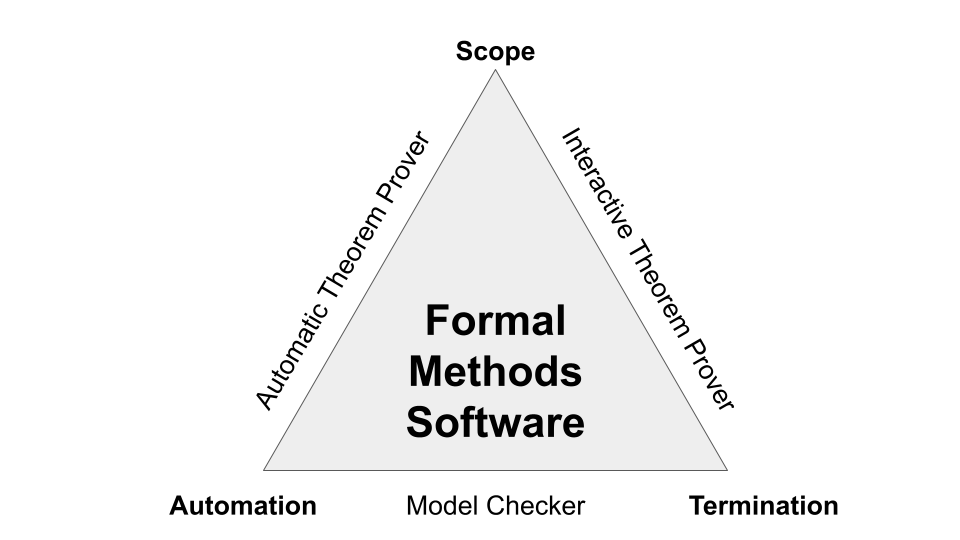
\includegraphics{./Images/formalmethods.png}
\caption{Three categories of Formal Methods}\label{fig:formal_methods}
}
\end{figure}

\textbf{Features of Formal Methods Tools:}

\textbf{Automation}: Whether finding a proof is fully automated. That
is, the user does not need to specify a proof manually for the
proposition, the system simply attempts to find one automatically.

\textbf{Termination}: Whether the tool terminates in a practical amount
of time when attempting to find a proof. For instance, does not have the
possibility of running for several days when attempting to prove a
proposition.

\textbf{Scope}: Whether the tool is able to prove any arbitrary property
about a system. The properties that can be proven are not restricted to
a subset of possible properties.

\textbf{Formal Methods Tools:}

\textbf{Model Checkers} are fully automated and if the specification is
not particularly large, can find solutions in a reasonable amount of
time. However, Model checkers can do this by restricting the scope of
the systems that they can prove. They allow for a specification for a
system in a (usually finite) state machine or automaton, and can prove
properties about this state machine. This means that you can only prove
with a model checker some simplification of the actual system, and often
cannot prove more complicated properties such as those with numbers.
This means that not all properties about the system can be verified.

\textbf{Automated Theorem Provers} (ATPs) are fully automated and can
prove arbitrary theorems, however may not terminate in reasonable time.
For larger systems or more complicated theorems, they may run forever
and never identify a proof or disproof for the proposition.

\textbf{Interactive Theorem Provers} terminate in reasonable time and
can prove arbitrary theorems. However, they are not fully automated, and
require the user's input to guide the proof of the theorem. This is a
major limitation as interacting with a human is often relatively slow
and expensive. Especially if the propositions that are being proven are
more trivial and could be solved quickly with an ATP.

The distinction between ATPs and ITPs is however not clear cut. ATPs can
often include minor user interaction in order to correct it's path and
find a proof. And ITPs often have automatic features and can even call
external ATPs to help automatically prove goals.

ITPs were chosen for this investigation due their usage in creating
fully certified software
{[}\protect\hyperlink{ref-CertifiedSoftware}{77}{]}. Model checkers can
be used to check important properties about software, but can't get the
last mile to make it fully certified due to not allowing the user to
prove all the propositions that might be relevant to the code. As
reliance on technology is only getting greater, it's important to
consider making technology as trustworthy as possible, particularly if
the software is safety/security-critical.

That being said, ATPs are often used beside ITPs, where an ITP might
call an ATP to prove a proposition or discover a counterexample
automatically. The primary goal in the development of ATPs is the speed
at which it can prove a variety of theorems. As of such, development of
ATPs directly influences development of ITPs by improving some of the
automation related tools in ITPs.

\hypertarget{sec:interaction_paradigms}{%
\subsection{ITP Interaction Paradigms}\label{sec:interaction_paradigms}}

ITPs can go about proving and specifying properties about software in
different ways. This section outlines a short history of interaction
paradigms with ITPs, and possible developments.

Direct Manipulation ITPs such as KeY work by editing proof objects until
the obligations have been resolved. These provers often have issues with
tedious interactions, and work has even been done add textual elements
to KeY {[}\protect\hyperlink{ref-beckert_interaction_2017}{16}{]}. The
development of interfaces to Direct Manipulation provers often differs
from textual ones.

Textual ITPs such as HOL, Isabelle, Coq and Matita work by writing a
proof script that attempts to prove a proposition. Interacting with
textual ITPs often involves a very simple read-evaluate-print-loop
(REPL) for their interfaces. This is very similar to the example we went
through in section Section~\ref{sec:using_an_itp}. One very stark
example of this is HOL-Light, which the user interacts with by opening
up the OCaml REPL (a general purpose ML based functional programming
language) and loading the HOL library. All OCaml is available alongside
the HOL library. Although this is rather primitive, modern ITP
interfaces such as Isabelle/jEdit and CoqIDE usually offer only a small
layer of abstraction over a REPL for their own languages.

These interfaces have two main windows, the first has code and the
second has proof state. The code can be evaluated up to a certain point,
and the output from the REPL in terms of proof state are printed in the
second window. The only major difference between this and a standard
REPL is that the user can rewind to evaluate up to a previous line. This
simple style of interface has consequences for usability. In particular,
if any error is found either in proof or in syntax, execution stops
until that error is resolved. Further, for larger projects, it can take
a very long time for systems to recompile. It also means that the user
can only reference things that have already been declared (it has to be
a single pass). This is particularly an issue when automated tactics
attempt to use lemmas above them to find solutions to theorems (such as
Isabelle). This means that simply changing the order of lemmas in an
Isabelle document, even if they never reference lemmas that are below
them, could cause a lemma that was proven before to become unproven.

Developments in IDEs to allow asynchronous interfaces, reloading only
parts needed and loading proofs out of order have been introduces to fix
this problem. They are called "Prover IDEs", with two examples being
Isabelle/PIDE~{[}\protect\hyperlink{ref-wenzel_asynchronous_2014}{82}{]}
and Coq/PIDE~{[}\protect\hyperlink{ref-barras_asynchronous_2015}{10}{]}.
These hopefully will resolve some of the issues cited above.

Although we have examples of large projects undertaken with ITPs,
optimal interaction paradigms are still up for debate, and several novel
interaction paradigms have surfaced. Including proving theorems and
writing tactics with
diagrams~{[}\protect\hyperlink{ref-grov_tinker_2018}{38},
\protect\hyperlink{ref-lin_understanding_2016}{55},
\protect\hyperlink{ref-shams_accessible_2018}{76}{]}, or providing agent
based
interfaces~{[}\protect\hyperlink{ref-hunter_agent-based_2005}{46}{]}.

We now move into the usability problems and solutions found in ITPs.

\hypertarget{sec:using_an_itp}{%
\subsection{Using an ITP}\label{sec:using_an_itp}}

To explain the typical terms and issues related to ITPs, let us present
an small toy example of using an ITP using pseudocode syntax.

Our pseudocode syntax is based on textual ITPs such as Isabelle, Coq and
HOL. The syntax is simplified to get the basic concepts of ITPs across
without too many of the technical details.

To prove a property with an ITP, the user must start by having a goal
that they wish to prove. You then manipulate and decompose that goal
into simpler subgoals, until they've proven the proposition they wish to
prove.

We start with a function:

\[
f(x) = 
  \begin{cases}
    f(x - 1) + x, & x > 0 \\
    0, & x = 0
  \end{cases}
\]

This is the triangle number function. It adds a number to every number
below that number up until 0. For instance,
\(f(5) = 5 + 4 + 3 + 2 + 1 + 0 = 15\).

However, there is a quicker way to calculate the triangle number, and
that is that is that \(f(x) = \frac{x(x + 1)}{2}\).

This proof is an elementary induction proof. But we shall demonstrate
that this statement is true.

We would like to prove that:

\[ f(x) = \frac{x(x + 1)}{2} \]

Textual ITPs are similar to interactive programming languages, such as R
and Bash, where the main interaction is through a Read Evaluate Print
Loop or REPL. You start by writing a line of code, and the ITP will
return the state. These lines of code manipulate the state until the
statement has been prover. After the proof, the user is left with a
proof script, which is a listing of all the code used to prove the
proposition.

To start with our proof, we first have to specify the property that we
wish to prove. In pseudocode, we write Listing~\ref{lst:proposition}
into our ITP. This statement says that the user would like to
\passthrough{\lstinline!Prove!} the statement
\passthrough{\lstinline!forall x, f(x) = x * (x + 1) / 2!}.
\passthrough{\lstinline!Prove!} here is a keyword that starts the proof.
Everything between the \passthrough{\lstinline!:!} and the
\passthrough{\lstinline!.!} represent the statement they wish to prove.

\begin{lstlisting}[caption={User Input: Statement of the proposition to prove}, label=lst:proposition]
Prove: forall x, f(x) = x * (x + 1) / 2.
\end{lstlisting}

After writing this statement, the ITP will print the display shown in
Listing~\ref{lst:starting_state}. This will often appear in a window in
the ITP interface, or if it is a command line prover, it will print it
to console.

The state is separated into two sections, everything above the
\passthrough{\lstinline!---!} is an assumption, that is, what we have
assumed to be true. We can have multiple assumptions, but in this case,
there are none. Then the statement below the
\passthrough{\lstinline!---!} is the \textbf{goal}. This is the
statement to prove. When starting a proof, whatever statement the user
wishes to prove becomes the first goal, but both the assumptions and the
goal will change as the user progress in the proof. It's also possible
to split the goal into multiple subgoals as the proof is being
developed.

\begin{lstlisting}[caption={ITP Output: Starting state}, label=lst:starting_state]
---
forall x, f(x) = x * (x + 1) / 2
\end{lstlisting}

Now we must give a series of \textbf{tactics} to the ITP to prove this
proposition. A tactic is like a command that is sent to the ITP in order
to prove the proposition that you wish to prove. Tactics are always
typed, and sometimes they fail to work in situations where their usage
would be invalid. These tactics form a language that you can use to
specify your proof.

It should be noted that while attempting to prove a proposition, the
user may wish to attempt to prove a goal or subgoal automatically. Most
ITPs have the ability to automatically prove simple propositions, often
by giving the \passthrough{\lstinline!auto!} tactic to the prover. If
this succeeds, then the user is done and the proposition is proven.
Otherwise, the user must continue to explore proof options. Furthermore,
the ITP can assist the user by offering counterexamples to why the
proposition might not actually be true. We will assume that the
statement cannot be proven automatically.

This particular proof is often used as an introductory induction proof,
so induction would be a good start to solving this. Entering the
pseudocode in Listing~\ref{lst:induction_tactic} performs induction on
the variable x. To perform induction, we must prove the base case, and
then prove the inductive case. The ITP will ask to prove them one at a
time, starting with the base case. After the tactic is executed, the
state of the ITP will be modified, and display the state in
Listing~\ref{lst:induction_state}.

The state has now been split up into two \emph{subgoals}. One for the
base case and one for the induction case, which is labeled as (1/2). In
our pseudocode ITP, all the tactics that we write will manipulate the
first goal only, but the ITP is indicating that there still is a second
goal that needs to be proven after this first one. This means that the
theorem prover is asking for a proof of the base case, that is, that the
statement is true when \(x = 0\).

\begin{lstlisting}[caption={Running the induction tactic}, label=lst:induction_tactic]
induction x
\end{lstlisting}

\begin{lstlisting}[caption={State after the induction tactic}, label=lst:induction_state]
---
f(0) = 0 * (0 + 1) / 2
(1/2)
---
f(x) = x * (x + 1) / 2 -> f(x + 1) = (x + 1) * (x + 2) / 2
(2/2)
\end{lstlisting}

Notice that the tactic modifies the state of the ITP. Only tactics that
are valid at the time are allowed to be used, ensuring that all proof
steps are valid and construct a correct proof.

The base case is very easy to solve, as simply evaluating the function
on both sides (\(f(0) = 0\) and \(\frac {0 \cdot (0 + 1)}{2} = 0\))
gives 0.

To evaluate this, we use the \passthrough{\lstinline!simplify!} tactic
in Listing~\ref{lst:simplify_tactic}. This tactic attempts to try a list
of rules that the prover guesses will simplify the current statement. In
our pseudocode ITP, this includes evaluating statements with constants.
The result is as we expect and shown in
Listing~\ref{lst:simplify_state}. Indicating that after the
simplification, both sides are equal to each other.

\begin{lstlisting}[caption={Running the simplify tactic}, label=lst:simplify_tactic]
simplify
\end{lstlisting}

\begin{lstlisting}[caption={State after running the simplify tactic}, label=lst:simplify_state]
---
0=0
(1/2)
f(x) = x * (x + 1) / 2 -> f(x + 1) = (x + 1) * (x + 2) / 2
---
(2/2)
---
\end{lstlisting}

Now the goal is to prove that \passthrough{\lstinline!0=0!}. This is
trivially true because equality is reflexive. As of such, we can prove
the current goal by indicating that it's reflexive. We can use the
\passthrough{\lstinline!reflexivity!} tactic to prove any goal that is
true because of reflexivity. This tactic is executed in
Listing~\ref{lst:reflexivity_tactic}.

After we have solved the first goal, the base case, the pseudo-ITP is
now asking us to prove the inductive case in
Listing~\ref{lst:reflexivity_state}. The current goal is now to prove
the inductive case. As it is with induction, the inductive case allows
us to assume that the original proposition is true for any x, and that
we need to prove that it is the case for x + 1. Therefore, the statement
for proposition for (x + 1) is our goal.

\begin{lstlisting}[caption={Running the reflexivity tactic}, label=lst:reflexivity_tactic]
reflexivity
\end{lstlisting}

\begin{lstlisting}[caption={State after running the reflexivity tactic}, label=lst:reflexivity_state]
f(x) = x * (x + 1) / 2
---
f(x + 1) = (x + 1) * (x + 2) / 2
\end{lstlisting}

The first step would be to replace \passthrough{\lstinline!f(x + 1)!}
with it's definition. This can be done with the
\passthrough{\lstinline!unfold!} tactic, as shown in
Listing~\ref{lst:unfold_tactic}. This tactic replaces a function with
it's definition. This replacement is shown in
Listing~\ref{lst:unfold_state}

\begin{lstlisting}[caption={Running the unfold tactic}, label=lst:unfold_tactic]
unfold f
\end{lstlisting}

\begin{lstlisting}[caption={State after running the reflexivity tactic}, label=lst:unfold_state]
f(x) = x * (x + 1) / 2
---
f(x) + (x + 1) = (x + 1) * (x + 2) / 2
\end{lstlisting}

Our current assumption and the goal are equivalent statements in
different forms. We now have to re-arrange the goal to make it equal to
the assumption. This might involve several tactics to manipulate the
state of the equation. We will for the sake of brevity written these
tactics in English like code in Listing~\ref{lst:rearangement_tactics}.
The intermediate goals are shown in
Listing~\ref{lst:intermediate_states} to show the progress towards the
desired goal, and the final state is shown in
Listing~\ref{lst:rearangement_state}.

\begin{lstlisting}[caption={Running re-arangement tactics}, label=lst:rearangement_tactics]
expand (x + 1) * (x + 2)
subtract both sides (x + 1)
replace (x + 1) with (2 * (x + 1) / 2)
combine fraction
simplify
factorise (x * x - x)
\end{lstlisting}

\begin{lstlisting}[caption={States after running each tactic}, label=lst:intermediate_states]
f(x) + (x + 1) = (x^2 + 3x + 2) / 2
f(x) = (x^2 + 3x + 2) / 2 - (x + 1)
f(x) = (x^2 x + 3x + 2) / 2 - ( 2 * (x + 1) / 2)
f(x) = (x^2 + 3x + 2 - 2 * (x + 1)) / 2
f(x) = (x^2 + x) / 2
f(x) = x * (x + 1) / 2
\end{lstlisting}

\begin{lstlisting}[caption={Final state after running each tactic}, label=lst:rearangement_state]
f(x) = x * (x + 1) / 2
---
f(x) = x * (x + 1) / 2
\end{lstlisting}

Because we know the inductive hypothesis is true, and the goal is
exactly the same as the inductive hypothesis, we can simply indicate
that we have proven the goal. We do this be the
\passthrough{\lstinline!assumption!} tactic, and then close off the
proof with the \passthrough{\lstinline!QED!} tactic
Listing~\ref{lst:assumption_tactic}. This then accepts the proof as true
Listing~\ref{lst:assumption_state}.

\begin{lstlisting}[caption={Running the assumption tactic}, label=lst:assumption_tactic]
assumption
QED
\end{lstlisting}

\begin{lstlisting}[caption={State after running the assumption tactic}, label=lst:assumption_state]
Proof accepted
\end{lstlisting}

It should be noted that the tactic we wrote out are akin to deduction
rules, however, there is a problem with this approach, and the problem
should become clear once we write down all the commands that have been
put into the prover.

\begin{lstlisting}[caption={Final Proof script}, label=lst:final_proof_script]
Prove: f(x) = x * (x - 1) / 2
introduce
induction x
simplify
reflexivity
unfold f
expand (x + 1) * x
subtract both sides x
replace x with (2 * x / 2)
combine fraction
replace ( + x - 2 * x) with ( - x)
factorise (x * x - x)
assumption
QED
\end{lstlisting}

These proof scripts are very difficult to understand statically, that is
it's difficult to formulate the reasoning behind the proof simply by
looking at the list of tactics that were used to prove the proposition.
Our understanding of the tactic were aided due to our knowledge of the
current state, and understanding However, when looking at the script
without the context of the state, they are often very difficult to
follow. Especially if the scripts are more complicated than this one.

\hypertarget{cognitive-dimensions}{%
\subsection{Cognitive Dimensions}\label{cognitive-dimensions}}

Usability problems with ITPs have been noted in the past. In particular,
it was completed as part of Kadoda's PhD thesis in 1999
{[}\protect\hyperlink{ref-kadoda_formal_1997}{49}{]}. In their thesis,
Kodada used Cognitive Dimensions of Notation to classify and sort
usability issues. With ITPs.

Cognitive Dimensions of Notation is a framework proposed by Green
{[}\protect\hyperlink{ref-green_usability_1996}{37}{]}, as a way of
discussing the design trade-offs of visual programming languages, but
has been applied elsewhere for a variety of notations. These dimensions
are not an evaluation framework for notations, as often increasing one
dimension will also change other dimensions, and different tasks may
require different dimensions. For instance, in textual ITPs,
dependencies are not shown between theorems, and doing so would increase
the Diffuseness of the notation, allowing less to be shown and
understood on a single screen. However, debugging why some theorem might
fail given a change in other theorems would aid from a more diffuse
representation showing the hidden dependencies.

Cognitive Dimensions focus mainly on the way that users understand and
work with the meaning of the program. Cognitive Dimensions make an
important distinction between difficulties of understanding and working
with the notation vs.~difficulties with the actual problem itself.
Because proving theorems is a very cognitively demanding task, and a lot
of that difficulty is inherit to the problem of proving theorems, and no
amount of notation will solve it. As of such, we need to focus on ways
that the notation can be improved to remove as many difficulties as we
can that are not inherit.

Cognitive Dimensions of Notations has been adopted as a way of
evaluating the usability of ITPs in Kadoda PhD
thesis~{[}\protect\hyperlink{ref-kadoda_desirable_1999}{50}{]}. In their
thesis, they simply use the dimensions as a framework for constructing a
questionnaire about possible usability issues with ITPs. We derive our
definitions of Cognitive Dimension as applied to ITPs from her thesis.

This thesis will be using Cognitive Dimensions of Notations framework to
classify different usability problems. The Cognitive Dimensions of
Notations and their definitions are presented:

\textbf{Abstraction Gradient}: Does the ITP offer ways of abstracting
components? Abstraction here refers to methods, classes and
encapsulation. Green classifies notations as either being
abstraction-hating, abstraction-tolerant or abstraction-hungry. An
abstraction-hating ITP would be one that forces the user to work with
low level constructs often. An abstraction-tolerant ITP would be one
that gives some methods for abstraction, but still nevertheless requires
constant low level interaction. An abstraction-hungry ITP would offer
many methods of abstraction, that could even in the end obscure what is
actually happening behind the scenes.

\textbf{Closeness of Mapping}: Closeness of Mapping is how similar the
notation is to the problem domain. At some point, a representation of
the problem has to be put into notation suitable for the ITP. The easier
this is to do the better the closeness of mapping, or how close the
proof state is represented vs what the user would expect.

\textbf{Consistency}: Once the user know the basics of an ITP, how much
of the rest can be inferred? A notation that is not consistent would
require constant lookup of features in the theorem prover. Consistency
is particularly important for learning ITPs. Consistency can become an
issue when there are a large amount of abstractions.

\textbf{Error-Proneness}: Is it easy to make careless mistakes? A common
"careless mistake" in theorem provers is trying to apply a tactic in a
textual theorem prover that is not valid for the current proof state.

\textbf{Diffuseness}: How much does it represent a proof relative to the
complexity of the proposition proven? This is an easier cognitive
dimension to measure, and represents the verbosity of the notation. ITPs
with high diffuseness often have lower abstractions and are easier to
understand, but more difficult to change.

\textbf{Hard Mental Operations}: Are there parts of the notation that
require getting out a pencil and paper to understand what it means? The
domain of ITPs by it's very nature requires Hard Mental Operations, so
it's important to separate the inherit difficulty vs difficulty created
by the notation. Hard Mental Operations may arise out of particularly
complicated tactics, especially since tactics can be composed together.
An ITP with a consistent set of tactics would reduce Hard Mental
Operations.

\textbf{Hidden Dependencies}: Are there dependencies in the notation
that are not presented? In ITPs and programming languages, it's usually
possible to find what a function/lemma references, but is difficult to
find what lemmas/functions reference the one we are working in.
Furthermore, automation often uses lemmas in the context without
indicating at all that it is using them. This makes the issue of hidden
dependencies even more difficult. An ITP with low hidden dependencies
makes these dependencies between parts of the program explicit

\textbf{Perceptual cues}: Does the notation force the user to make
decisions before they have the information they need to make it?
Especially for novice users, ITPs need to allow the user to explore
different paths for proving a statement. This often represents a
premature commitment as the user has to commit to a strategy before
evaluating whether that strategy would work. ITPs that offer undo
features and allow postponing making decisions require less premature
commitment.

\textbf{Premature commitment}: Does the notation force the user to make
decisions before they have the information they need to make it?
Especially for novice users, ITPs need to allow the user to explore
different paths for proving a statement. This often represents a
premature commitment as the user has to commit to a strategy before
evaluating whether that strategy would work. ITPs that offer undo
features and allow postponing making decisions require less premature
commitment.

\textbf{Progressive Evaluation}: Does the system give adequate feedback?
Error messages, display of current proof state and ability to work with
incomplete proofs are all features of progressive evaluation. Getting
feedback from the system is absolutely essential for learning the ITPs.

\textbf{Role Expressiveness}: Is it easy to identify what the purpose of
a component is? Lack of role expressiveness, particularly within the
proofs of textual ITPs, was one of the main motivations of this study.
It is often very difficult on retrospect to identify how the components
of a proof relate to each other. An ITP with high Role Expressiveness
would make it clear how a lemma or component of a proof contributes to
the proof.

\textbf{Secondary Notation}: Are there avenues for comments, colours and
representation of the code that helps with comprehension? A Secondary
Notation is a way of representing understanding by not changing the
actual meaning of the notation. ITPs that offer comments, colours and
whitespace grouping help with representing secondary notation.

\textbf{Viscosity}: Is it easy to make a change in the system? ITPs with
low abstraction make it difficult to make changes. Sometimes a small
difference to what the user is wanting to prove requires a
disproportionate change of the proof. ITPs with high viscosity make it
difficult to change.

\textbf{Visibility and Juxtaposability}: How easy is to get a particular
piece of desired information? How easy is it to compare part of the
proof with proofs elsewhere? Sometimes critical information is difficult
to obtain when creating or understanding a proof state. A common example
is being able to inspect intermediate proof steps. When a proof relies
heavily on automation, it is sometimes difficult to understand how the
automated tactic managed to get in a particular proof state. Having this
information helps understand the proof and how to move forward. ITPs
with low visibility make it difficult to find such information.
Juxtaposability is showing two parts of the system side by side. This is
important as often a proof might only be a refinement of a previous
proof, and might need to be understood in context.

\hypertarget{research-questions}{%
\subsection{Research Questions}\label{research-questions}}

This thesis was inspired by the difficulty in reading static proof
scripts. Some provers have already moved to attempt to fix this problem.
For instance, Isabelle's Isar language offers a different way of proving
propositions that embeds more state, and helps the user understand the
proof. It would be therefore valuable to determine what usability issues
have been reported, what has been done to fix them, and whether
solutions from some ITPs could be used to help other provers.

And finally, the secondary motivation of this thesis is to encourage
further use and development of ITPs. So it would be valuable to create a
decision tool that helps a user determine which ITP, if any, should be
used for a particular project.

Hence, the research questions for this thesis are:

RQ1 \emph{What usability issues and solutions have been mentioned in
literature regarding ITPs?}

This research question was chosen to better understand the context of
the study. This was answered by a systematic literature review in
Section~\ref{sec:literature_review}.

RQ2 \emph{To what extent to these usability issues exist at the latest
versions of ITPs?}

This research question was chosen due to the continual development of
ITPs. It is answered by a living review in Section~\ref{sec:results}.

RQ3 \emph{What, if any, ITP should be used for a specific project?}

Finally, this research question was chosen as being important for the
aim of encouraging more development in the field of ITPs and the
creation of more verified software. It is answered by a living review in
Section~\ref{sec:results}.

\hypertarget{methodology}{%
\section{Methodology}\label{methodology}}

In this section, we go over the methodology for answering our research
questions. We will structure our systematic literature review, and
outline our contribution of a separate living review.

The natural method for answering RQ1 is to perform a systematic
literature review. This literature review intends to identify and
categorize usability issues related to different theorem provers. We
outline the methodology for this review in
Section~\ref{sec:review_methodology}.

Answering RQ2 requires going through the theorem provers and identifying
the issues. However, ITPs are continually in development, and any issue
that arises could be solved at a future date. As of such, we created a
\textbf{living review} to answer this question.

A living review is a literature review of a field that updates
periodically to reflect the current state of the research. These reviews
are often published electronically, such as to a website. The goal of a
living review is to ensure that the review never goes stale, and can be
used as a reference years to come.

Our review looks through more than just literature, and attempts to
directly track progress towards fixing usability problems in ITPs. The
methodology for the living review is detailed in
Section~\ref{sec:living_review_meth}.

This living review is the primary output of this thesis, and although it
has the word ``review'' in it, should not be mistaken for just another
literature review.

It differentiates itself from a normal review by updating automatically
over time, being an interactive software product, and existing as a
decision tool for users.

The creation of this living review will answer RQ3 and RQ2, and provide
descriptions of the current state of the field for ITPs.

\hypertarget{sec:review_methodology}{%
\subsection{Systematic Literature Review
Methodology}\label{sec:review_methodology}}

A preliminary literature review was done in order to survey what
usability problems occurred about theorem provers. This preliminary
review came from a search for ``usability interactive theorem provers"
on the ACM digital library and Google Scholar. The review found several
papers on the topic. We then attempted to construct a query that would
match these papers and also other papers in the field.

Papers were searched for having the title matching the following query:
\passthrough{\lstinline!("Interactive" OR "Deductive") AND ("prover" OR "provers" OR "proving" OR "verifier") AND ("usability" OR "user" OR "users")!}

The justification for using quotes around prover, provers and proving is
that some search engines will return papers with the text "prove" when
looking for "prover". "prove" therefore comes up with many more records
that are unrelated to our topic. "Usability" is also quoted to prevent
searching for "use", which clearly would bring in papers that are
unrelated.

We searched the following databases using this query string:

\begin{itemize}
\tightlist
\item
  Scopus
\item
  DBLP
\item
  Springer Link
\item
  Science Direct
\item
  ACM
\item
  IEEE
\item
  Xplore
\end{itemize}

From the papers discovered in this way, we went through the abstracts
and discerned whether the paper was relevant to the research question.

Our inclusion criteria for the papers inclusion and exclusion criteria
in the systematic literature review were the following:

\begin{itemize}
\tightlist
\item[LIC1]
  A peer review published paper.
\item[LIC2]
  Notes particular usability issues with theorem provers OR\\
  Offers direct recommendations to the improvement of the usability of
  interactive theorem provers.
\item[LEC1]
  The paper is written in a lanugage other than english
\item[LEC2]
  The paper is of a tutorial, workshop, extended abstract.
\item[LEC3] the item is not peer reviewed.

\item
\end{itemize}

From the papers that were deemed relevant to the research question, we
found papers that cited the papers discovered. That is, we applied
forward snowballing {[}\protect\hyperlink{ref-Snowballing}{86}{]}.
Semantic scholar was used to perform the forward snowballing.

We then tried to discover whether these papers were relevant to the
research question, and repeated the process of forward snowballing until
there were no more papers discovered.

We then analysed the identified papers to discover:

\begin{itemize}
\tightlist
\item
  A problem and/or solution to usability of interactive theorem provers
\item
  Which theorem prover the issue is relevant to
\item
  Evidence behind issues and proposed solutions
\end{itemize}

The issues were then categorized by Green's Cognitive Dimensions of
Notations~{[}\protect\hyperlink{ref-green_usability_1996}{37}{]}. This
literature review therefore will answer RQ1.

\hypertarget{sec:living_review_meth}{%
\subsection{Living Review Methodology}\label{sec:living_review_meth}}

The living review has the end goal of determining whether usability
issues still exist, and then further offering a tool to help decision
about ITPs (RQ3).

The following sections describes the methodology in detail. First, we
discuss the choice of Interactive Theorem Provers included within the
review in Section~\ref{sec:chosing_itps}. Then, we discuss the
methodology used in evaluating the scope of the library in
Section~\ref{sec:scope_of_library_meth}. Then, we discuss the
methodology for evaluating support for counterexample generators in
Section~\ref{sec:counterexample_meth}. Finally, we discuss the
methodology for evaluating support for math notation in
Section~\ref{sec:math_notation_meth}.

\hypertarget{sec:chosing_itps}{%
\subsubsection{Choosing Interactive Theorem Provers to
Cover}\label{sec:chosing_itps}}

In this section, we discuss the choice of which ITPs to cover as part of
the living review.

A reasonable approach to this would be to reference a past review and
borrow their scope of ITPs. This was done with
{[}\protect\hyperlink{ref-nawaz_survey_2019}{63}{]}. The ITPs in this
review include Isabelle, Coq, HOL, Agda, PVS, LEO-II, Watson, Yarrow,
Atelier B, Metamath, Twelf, Mizar, RedPRL, JAPE, LEO-II, Getfol, and
Z/EVES.

However, we noted a couple of issues with this consideration of ITPs. In
particular, it seemed to favour reviews of older ITPs, and didn't
include successful ITPs that have come out more recently.

One clearly missing consideration was that of Lean
{[}\protect\hyperlink{ref-Lean}{61}{]}, a highly popular ITP that's more
often used by mathematicians. Lean is mentioned within the review as a
`newer ITP' but is not considered as part of the review. We chose to add
Lean, particularly because of its large community based mathematical
library. It would be difficult to make a comparison between mathematical
libraries, as we intend to do, without including this one, due to being
particularly large.

Secondly, there were some provers that were included within this review
that are currently abandoned. Those two provers were Yarrow, and Watson.
These two provers had their last releases in 1999 and 2001. Considering
the rate of development of ITPs, these were removed due to meeting a
very conservative definition of being abandoned.

Finally, the last modification that was made was that the survey
referenced ``HOL'' as a theorem prover. HOL has many implementations,
including HOL4 {[}\protect\hyperlink{ref-HOL4}{78}{]}, HOL Light
{[}\protect\hyperlink{ref-HOL_Light}{41}{]}, ProofPower
{[}\protect\hyperlink{ref-ProofPower}{70}{]} and HOL Zero
{[}\protect\hyperlink{ref-HOL_Zero}{2}{]}. For the sake of this review,
keeping these separate was appropriate as only properties of different
theorem provers were discussed, and these properties remained largely
the same for each implementation. However, because this living review
covers mathematical libraries, it will require comparing between
implementations. As of such, ``HOL'' was split into its two most popular
interventions, HOL4 and HOL Light. These two were chosen as they have
decently sized mathematical libraries, whereas HOL Zero and ProofPower
do not. Including HOL Zero or ProofPower would therefore not add much
value to the living review.

\hypertarget{sec:scope_of_library_meth}{%
\subsubsection{Scope of Library}\label{sec:scope_of_library_meth}}

This section reviews the methodology for investigating the scope of
libraries within the living review.

In a focus group\textasciitilde{}\cite{beckert_usability_2015}, it was
found that Isabelle/HOL was missing important mathematical foundations
in their library.

We decided to evaluate whether these problems still exist by evaluating
the scope of library support of ITPs. We have the goal of determining
whether mathematical foundations were covered, and by which provers they
are covered by.

On a high level, the mathematical libraries for different ITPs will be
decomposed into modules, and each of these modules are classified
according to which section of mathematics they cover. This way we can
identify which ITPs cover which mathematical topics, and make meaningful
comparisons between them.

\begin{figure}
\hypertarget{fig:classification_summary}{%
\centering
\includegraphics{Images/summary.png}
\caption{Flow chart for classifying mathematical
libraries}\label{fig:classification_summary}
}
\end{figure}

The flowchart shown in Figure~\ref{fig:classification_summary} has an
overview of the methodology to be used used to evaluate the scope of the
mathematical libraries.

\hypertarget{sec:identifying_math_lib_meth}{%
\paragraph{Step 1: Identifying Mathematical
Libraries}\label{sec:identifying_math_lib_meth}}

We start by identifying mathematical libraries. For the sake of this
analysis, we also include community contributions, such as package
management systems, as part of the scope. As of such, a ``library'' will
refer to both a library that comes along with an ITP (often titled a
``standard library'') as well as a collection of community
contributions, such as package management system.

A ``module'' from a library may refer to different things, including a
``package'' in some systems or a collection of code files.

For each ITP, it will be determined whether they first had a body of
code similar to a library. If it did, then it was determined whether the
library simply meets the following inclusion criteria:

\textbf{IC1:} The library contains mathematical theorems. Libraries that
do not prove theorems are often libraries that are about simple
constructions of data types.

\textbf{IC2:} The library contains more than 15000 lines of proof code
worth of math theorems. This, as identified later, corresponds to about
10 modules. If the library doesn't offer that many modules, then we
consider this to not be of interest to a mathematician.

or each ITP, it is determined whether they had a collection of community
maintained contributions. These community contributions are included if
they were collected and listed in some freely available place on the
internet. This is done to ensure that when the list of contributions
changes or expands, this living review could be updated.

\hypertarget{sec:collecting_modules_meth}{%
\paragraph{Step 2: Collecting
Modules}\label{sec:collecting_modules_meth}}

The next step is to determine what constituted a module for each of the
libraries. We define a \textbf{module} as a single unit of work
contributed to an ITP. This is used to reason about contributions and
the scope of the ITP. We define this concept as in our analysis we cover
both components of standard libraries, and packages in package
management systems.

If the module came from a community contribution, for instance,
Isabelle's archive of formal proofs or Coq's package management system
then it is considered a ``package'' type. Meaning a module is considered
to be whatever a unit of contribution is. For instance, a package is
considered a module in Coq's package management system, or a submission
in the Archive of Formal Proofs. We consider this to be a natural
mapping because there is very little other options in defining a module
in a package management system. It would both be unusual to split up
packages into their smaller components due to having non standardised
structure and also unusual to define a module as a collection of
packages. It also means that the module is understandable, linkable and
explorable in the review.

If the modules came from a ``standard library,'' we attempted to divide
the standard library into ``package sized'' sections, in order to make a
fair comparison between contributions. Because a package, as above, is a
natural mapping to modules, and standard libraries are often much larger
than a single package, we need to split the library up in a way that
makes it comparable to a package. To do this, we exploited that most
libraries are structured in a hierarchy, so we split the library as
determined by how far down the hierarchy we need to go until we get
``package sized'' sections. If only one level of the hierarchy is
needed, it is classified as ``small,'' if two levels are needed, it is
classified as ``large.''

To determine whether a library is small or large, we first have a target
module size, which we define to be 1500 lines of proof code. The exact
number is based off sizes of HOL Light modules, which are considered a
minimum exposition of a topic to be considered a module. Then, the mean
module size is calculated, and it is determined whether a small or large
library is closer to 1500 lines on a log scale.

These modules are then collected from the website automatically from the
webpage using a python script. The script will be designed so that it
can update the review to newest modules automatically, ensuring that the
users are always viewing the most up to date version of these libraries.

From the modules, a number of elements were collected. The name of the
module, a description if it was available, authors if it was available,
and a URL to the module. These will all be presented to the user when
discovering different modules supported by different ITPs.

\hypertarget{sec:classifying_modules_meth}{%
\paragraph{Step 3: Classifying
modules}\label{sec:classifying_modules_meth}}

There are a number of exclusion criteria for this classification. These
exclusion criteria exist for modules that would be difficult or
impossible to classify as a part of a mathematical topic. Those possible
exclusion criteria include:

\textbf{EC1:} Utility, The module only offers a utility that is only
relevant to this ITP. For instance, many ITPs double as programming
languages, so any modules that allow for programming that works with the
system such as file operations are excluded. This also includes modules
that are integrations with other tools, or simply initialization
libraries that only reference other modules.

\textbf{EC2:} No Documentation, If the module doesn't have any
documentation or description of purpose, it is excluded from the
classification. It should be noted that the definition of documentation
is very minimal in this case. The module doesn't need to have much
documentation, one sentence of its purpose is enough. However, if it is
missing, the module is difficult to classify and is excluded.

\textbf{EC3:} Only Documentation: If the module is simply documentation
and doesn't provide any new resources, it is also excluded.

\textbf{EC4:} Deprecated: If the module has been marked or considered
deprecated, then it is excluded from

Excluded modules will be marked as excluded, and the reason for
exclusion placed in the living review.

If a module doesn't fall under any exclusion criteria, then the modules
is ready to be classified. Each module is then assigned a mathematical
subject that its relevant to.

The topics these modules were classified under come from the
Mathematical Subject Classification 2020 (MSC2020)
{[}\protect\hyperlink{ref-msc2021}{9}{]}. MSC2020 is a classification of
mathematical subjects that is often used for mathematics papers. Each
topic is given a code representing its classification, One such example
of a code is 68P05, the code for work about data structures. The code is
split up into three sections, the top level is represented by a top
level mathematical field, For instance, the 68 in 68P05 means that it's
in the field of Computer Science. To refer to the general field of
Computer Science, it is referred to is 68-XX, with the -XX meaning that
it could be anything under this field. The next level of classification
is represented by a letter. In this case, the P in 68P05 refers to
subclassification of ``Theory of Data'' under ``Computer Science.'' If
one wishes to refer to the mid level classification, then one can do so
like 68Pxx, by replacing the final two numbers with ``x''s. Finally, the
last two numbers represents the final level of classification. In this
case, the 05 refers to ``Data Structures'' under ``Theory of Data''
under ``Computer Science.''

Some further examples of MSC Classifications are:

\textbf{68Nxx}: Theory of Software

\textbf{68N15}: Theory of Programming Languages

\textbf{13-XX}: Commutative Algebra

\textbf{13Axx}: General commutative ring theory

\textbf{13A50}: Actions of groups on commutative rings; invariant theory

This classification is chosen in order to be familiar to mathematicians,
and ensure that modules can be classified with enough specificity.

If the module also comes with some form of category (for instance, Coq's
package management system allows adding categories to a package,
indicating the subject it covers, or large library modules use the top
level module as a category), then the classification of the package is
``guessed.'' This is done by mapping the category to a classification.
The module can be browsed and seen in the tree, but however is marked as
``unverified.'' If the module doesn't come with a category, then the
module is marked as ``unclassified.''

Then, a module's description (for instance, abstracts, package
descriptions, names) is inspected manually and a classification is given
to it. The package is then considered to be ``verified.''

Finally, there is a limitation in our study, in that a very large number
of mathematical topics have been covered by ITPs. As of such, there are
some subjects that would require a very wide and professional
understanding of the many facets and areas of mathematics in order to
classify correctly. Any package that is therefore outside of the ability
of the author to classify, is labeled as ``needs professional'' during
verification. However, these modules are at the very least categorized
vaguely into a top level MSC classification. For example, the author
doesn't have a strong understanding of partial differential equations,
so any package that is from the field of partial differential equations
is marked as so, but not classified with any specificity beyond that.

This means that modules can be placed into five different states:

\textbf{Unclassified}: meaning that the module is included in the
system, but the system does not have any idea of what math
classification it falls under.

\textbf{Unverified}: The module's classification has been guessed
automatically based on a category provided by the resource providing the
module. For instance, Isabelle's Archive of Formal Proofs categorizes
packages by topic in their index, and the classification of the module
is guessed based on this.

\textbf{Excluded}: The module has been inspected and meets one of the
exclusion criteria. This excluded package is not classified and removed
from the study.

\textbf{Needs Professional}: The package requires a professional
mathematician to classify correctly.

\textbf{Verified}: The package has been verified manually to be in the
correct classification. This is the final desired state of a module.

States that are \textbf{Unclassified} or \textbf{Unverified} represents
states that are incomplete. As in, at some later point, manual
intervention is required to ``complete'' the classification. The reason
why we discuss and include unclassified and unverified modules in the
analysis is that we would prefer to present all the resources available
with a prover to a viewer, even the newest resources, before a human
goes into the system to verify a package. The goal however, is to have
no or little packages in the unclassified and unverified state.

\hypertarget{sec:counterexample_meth}{%
\subsubsection{Counterexample Generator
Methodology}\label{sec:counterexample_meth}}

It was suggested that counterexample generators could help users
understand proof state
{[}\protect\hyperlink{ref-beckert_usability_2015}{15}{]}. When proving a
theorem, a counterexample generator attempts to find an example for
which the theorem does not hold. This helps the user better understand
when the theorem and the statement that they wish to prove.

A literature review was performed in order to identify counter example
generators, and the systems that they have support for were also
recorded.

This is a very minor contribution, but simply attempts to give a very
brief overview of support for counterexample generators for theorem
proving.

\hypertarget{sec:math_notation_meth}{%
\subsubsection{Math Notation Methodology}\label{sec:math_notation_meth}}

Finally, as another minor contribution, we include details about which
theorem provers use mathematical notation in proving theorems.

Determining whether an ITP uses mathematical notation in proofs can
easily be done by examining example proofs, and determining whether they
use math notation. Which ITPs support mathematical notation was further
included as a minor contribution to the living review.

\hypertarget{general-features-of-about-itps}{%
\subsubsection{General features of about
ITPs}\label{general-features-of-about-itps}}

To compare between different ITPs, we must first start by collecting
general features about them. This is tied in RQ3, as working out whether
an ITP should be used on a project will require having some general
information about it.

We decided to use a 2019 Systematic Literature Reviews on Theorem
Provers as our starting dataset
{[}\protect\hyperlink{ref-nawaz_survey_2019}{63}{]}. This review went
through 27 theorem provers and described the features that each prover
had. This was converted into a dataset and used to compare general
features.

This dataset contained several properties about ITPs, and properties to
compare between them.

The full set of properties we used from the dataset are:

\begin{itemize}
\tightlist
\item
  What the ITP is based on (Syllogism, Type Theory, Etc)
\item
  The logic of the ITP
\item
  The Truth value of the ITP
\item
  Whether it supports Set theory
\item
  Whether it has a library
\item
  What the ITPs calculus is
\item
  Whether the architecture is modular or monolithic
\item
  The programming language it's implemented in
\item
  Whether it has a GUI or CLI interfaces
\item
  The Platforms its supported on (Windows, Mac, Linux)
\item
  Whether it has an IDE
\item
  When it was first released.
\item
  Its latest release
\end{itemize}

A lot of these features (such as the logic, truth value etc) require
explanations as to what they refer to. These explanations will be
included within the tool. This allows people unfamiliar to the field to
learn what the components of ITPs are and why they are important.

Some newer ITPs were not included in the dataset, such as Lean, F* and
Idris. These were added manually to the dataset.

The systematic literature review we source our data from however, is
already out of date for the latest release of its provers. As of such,
we have a python script that automatically retrieves whether any newer
versions of a prover have been released by checking GitHub Tags. It gets
the latest tag to be published and adds that as the latest release on
the living review, ensuring that the review doesn't go out of date by
having newer releases.

\hypertarget{sec:literature_review}{%
\section{Literature Review}\label{sec:literature_review}}

The amount of papers found in each section of the review are shown in
Table~\ref{tbl:litresults}. This totals to 36 papers found on the topic.

There was a surprisingly small amount of papers caught by query in
comparison to snowballing. This is because many papers that discuss
usability issues about ITPs do not tackle the problem directly (28/38 of
the papers), but rather showcase a feature that has been coded into an
ITP interface. These features do indeed solve a usability problem
implicitly, and represent the bulk of the work on improving interfaces
for ITPs. However, comparatively little research has been done
identifying the issues with ITP interfaces and empirically comparing
these user interface modifications for merit (10/38 of the papers).

\hypertarget{tbl:litresults}{}
\begin{longtable}[]{@{}lll@{}}
\caption{\label{tbl:litresults}Literature review papers}\tabularnewline
\toprule
Round & Found & Relevant \\
\midrule
\endfirsthead
\toprule
Round & Found & Relevant \\
\midrule
\endhead
Query & 45 & 14 \\
Snowball 1 & 121 & 14 \\
Snowball 2 & 191 & 5 \\
Snowball 3 & 99 & 2 \\
Snowball 4 & 44 & 1 \\
Snowball 5 & 4 & 0 \\
Total & 504 & 36 \\
\bottomrule
\end{longtable}

When going through papers, it was interesting to find a large amount of
papers proposing user interface models, but not actually identifying the
problems that they solve, nor evaluating their effectiveness. In fact,
out of the 28 papers that showcased user interface improvements, only 2
papers evaluated the their interface improvement to without the
improvement~{[}\protect\hyperlink{ref-berman_development_2014}{18},
\protect\hyperlink{ref-hentschel_empirical_2016}{44}{]}. That there is
not enough empirical studies verifying usability issues has been cited
as an issue that needs to addressed in the
past~{[}\protect\hyperlink{ref-hahnle_deductive_2019}{39}{]}.

The following sections outline usability issues and solutions to those
issues. Tables are included outlining the usability issues mentioned. If
the same problem is mentioned in two papers, it is given two rows.

The theorem prover column refers to the theorem prover the usability
issue was found in. If the problem is a general comment ``General" is
written.''Textual" means a theorem prover that uses proof script to
solve theorems, such as Isabelle/HOL, Coq, Agda. ``Direct Manipulation"
means a theorem prover that uses direct manipulation to solve theorems,
such as KeY.

The discovered column indicates the evidence that that problem exists.
"Suggested" simply means that problem or solution was simply inferred or
has not actually been evaluated as effective. Other values indicate the
type of study that the paper used to observe or evaluate this problem or
solution.

\hypertarget{theorem-provers}{%
\subsection{Theorem Provers}\label{theorem-provers}}

First of all, a brief overview of the theorem provers is in order.

\hypertarget{key}{%
\paragraph{KeY}\label{key}}

KeY is a Direct Manipulation theorem prover, meaning that unlike Textual
theorem provers, does not prove theorems by writing proof scripts, but
instead works by modifying a proof object directly until all proof
obligations have been solved. KeY works by annotating Java programs with
preconditions and postconditions. These conditions are then fed into KeY
as proof obligations. KeY can act as a fully automatic prover, but also
allows the user to attempt to find a proof if the prover fails. KeY has
also formed the basis of KeYmaera and KeYmaera X, which are for proving
properties of hybrid systems.

\hypertarget{hol}{%
\paragraph{HOL}\label{hol}}

HOL is actually a family of theorem provers. Notably HOL4, ProofPower,
HOL Light and HOL Zero. HOL is one of the oldest provers in this list,
and HOL Light is known to be used as a lightweight prover, with a very
easily checkable kernel. HOL provers are textual, and have a simple type
system and use tactics to prove propositions.

\hypertarget{isabelle}{%
\paragraph{Isabelle}\label{isabelle}}

Isabelle (also known as Isabelle/HOL, but for this paper will remain as
Isabelle to prevent confusion) is one of the most popular theorem
provers. The prover has been used for the verification of the SeL4
prover, and exists as the state-of-the-art of ITPs. Isabelle like HOL
has a simple type system and is based of the Logic for Computable
Functions.

\hypertarget{coq}{%
\paragraph{Coq}\label{coq}}

Coq is another popular ITP that also supports a dependent type system.
It's based on the Calculus of (Co)Inductive Constructions, which was
designed specifically for Coq. Coq has been used to prove the four
colour theorem, and create the CompCert certified C compiler.

\hypertarget{matita}{%
\paragraph{Matita}\label{matita}}

Matita is a theorem prover based on Coq's Calculus of (Co)Inductive
Constructions, and was designed to address many of the pain points in
working with Coq. Matita is a much simpler prover that aims to present
the theorem prover as editing a mathematical library. As of such,
Matita's solutions to problems are often pain points in Coq
(mathematical notation, Tinycals etc).

There are a few other provers also in this review, such as iCon, CardiZ
and Dafny. These ITPs are often either coded as proofs of concepts (such
as iCon), or are no longer maintained (in the case of CardiZ or Dafny).
The problems raised by them however, are often relevant for current day
ITPs.

This is by no means a complete list of modern ITPs. Such compilations
have been done~{[}\protect\hyperlink{ref-nawaz_survey_2019}{63}{]}.
These are only the ITPs discussed in the papers found in the review.
There are notable ITPs that are missing from this list that caught us by
surprise, including Agda, Lean and Mizar.

\hypertarget{abstraction-gradient}{%
\subsection{Abstraction Gradient}\label{abstraction-gradient}}

The problems classified under abstraction gradient are shown in
Table~\ref{tbl:abstraction_gradient}.

\hypertarget{tbl:abstraction_gradient}{}
\begin{longtable}[]{@{}llll@{}}
\caption{\label{tbl:abstraction_gradient}Abstraction Gradient
Problems}\tabularnewline
\toprule
Theorem prover & Problems & Discovered & citation \\
\midrule
\endfirsthead
\toprule
Theorem prover & Problems & Discovered & citation \\
\midrule
\endhead
KeY & Interaction with low level logic & Focus Groups &
{[}\protect\hyperlink{ref-beckert_usability_2015}{15}{]} \\
Isabelle & Missing Library & Focus Groups &
{[}\protect\hyperlink{ref-beckert_usability_2015}{15}{]} \\
\bottomrule
\end{longtable}

The abstraction gradient dimension concerns itself with the highest and
lowest levels of abstraction that are presented. Are they at the
appropriate level of abstraction?

Issues in this dimension were uncommon. KeY was found to require
interacting on low level logic formulas consistently. Similar issues
with tedious interactions with KeY are mentioned in the viscosity's
section. No solutions were found or suggested to this problem, and it
has not been empirically tested.

Focus Groups {[}\protect\hyperlink{ref-beckert_usability_2015}{15}{]}
found that Isabelle's library lacks the appropriate mathematical
foundations. Interestingly, this is the only issue of this class and is
not mentioned elsewhere, often library issues are more about managing
and searching large libraries, which Matita attempts to handle, and
correct documentation of libraries. This has not been tested
empirically. Other than the implicit solution of providing better
library support for theorem provers, no solution has been provided for
this problem.

\hypertarget{closeness-of-mapping}{%
\subsection{Closeness of Mapping}\label{closeness-of-mapping}}

The problems classified under Closeness of Mapping are shown in
Table~\ref{tbl:closeness_of_mapping}.

\hypertarget{tbl:closeness_of_mapping}{}
\begin{longtable}[]{@{}llll@{}}
\caption{\label{tbl:closeness_of_mapping}Closeness of Mapping
Problems}\tabularnewline
\toprule
Theorem prover & Problems & Discovered & citation \\
\midrule
\endfirsthead
\toprule
Theorem prover & Problems & Discovered & citation \\
\midrule
\endhead
KeY & Unintuitive mapping between formula and program & Focus Groups &
{[}\protect\hyperlink{ref-beckert_usability_2015}{15}{]} \\
CardiZ & Cannot sketch out proofs & Questionnaire &
{[}\protect\hyperlink{ref-kadoda_cognitive_2000}{48}{]} \\
Coq & Cannot use mathematical notation & Survey &
{[}\protect\hyperlink{ref-berman_development_2014}{18}{]} \\
Coq & Cannot use mathematical notation & Suggested &
{[}\protect\hyperlink{ref-asperti_user_2007}{7},
\protect\hyperlink{ref-zacchiroli_user_2007}{87}{]} \\
\bottomrule
\end{longtable}

The dimension of Closeness of Mapping is whether the interface maps well
to the problem world. For interactive theorem provers, it has to do with
how well the proof state is understood in comparison to the actual
problem.

Focus groups {[}\protect\hyperlink{ref-beckert_usability_2015}{15}{]}
found that because KeY attempts to prove properties through annotations
and java source code, it can sometimes be difficult to see how this
proof state maps to the
program~{[}\protect\hyperlink{ref-beckert_usability_2015}{15}{]}. This
issue is not mentioned in any other source and not tested empirically.
No solutions have been suggested for this.

CardiZ, an ITP that can be used to prove properties of Z specifications,
found that the user could not sketch out proofs before an attempt
{[}\protect\hyperlink{ref-kadoda_cognitive_2000}{48}{]}. This is the
only paper on CardiZ, as CardiZ is not a popular prover. No solutions
have been suggested for this.

A common issue that came up with Coq was the inability to use
mathematical notation {[}\protect\hyperlink{ref-asperti_user_2007}{7},
\protect\hyperlink{ref-berman_development_2014}{18},
\protect\hyperlink{ref-zacchiroli_user_2007}{87}{]}. Notation issues are
problematic in ITPs. One one hand, theorem provers such as Isabelle and
Agda allow using mathematical notation in their theorems. This helps the
user understand the theorem in a terse syntax. On the other hand,
mathematical notation can often be ambiguous and difficult to type.
Isabelle allows using LaTeX~style commands such as
\passthrough{\lstinline!rightarrow!} to render math notation, whereas
Agda allows Unicode in source files. In order to avoid ambiguity, Coq
has no support for math notation, and in response to this, Matita has
LaTeX~style mathematical
notation~{[}\protect\hyperlink{ref-asperti_user_2007}{7},
\protect\hyperlink{ref-zacchiroli_user_2007}{87}{]}. This issue came up
in three different sources.

\hypertarget{consistency}{%
\subsection{Consistency}\label{consistency}}

The problems classified under Consistency are shown in
Table~\ref{tbl:consistency}.

\hypertarget{tbl:consistency}{}
\begin{longtable}[]{@{}llll@{}}
\caption{\label{tbl:consistency}Consistency Problems}\tabularnewline
\toprule
Theorem prover & Problems & Discovered & citation \\
\midrule
\endfirsthead
\toprule
Theorem prover & Problems & Discovered & citation \\
\midrule
\endhead
Isabelle & Difficult to know what tactics and lemmas to use & Focus
Groups & {[}\protect\hyperlink{ref-beckert_usability_2015}{15},
\protect\hyperlink{ref-beckert_interaction_2017}{16}{]} \\
HOL & Difficult to know what tactic to apply next & Suggested &
{[}\protect\hyperlink{ref-aitken_interactive_1998}{3}{]} \\
Isabelle & Hard to remember prover specific details & Suggested &
{[}\protect\hyperlink{ref-nagashima_pamper_2018}{62}{]} \\
KeY & Difficult to know what tactic to apply next & Suggested &
{[}\protect\hyperlink{ref-mitsch_keymaera_2017}{59}{]} \\
Isabelle,HOL & Difficult to remember names of theorems & Observational &
{[}\protect\hyperlink{ref-aitken_analysis_2000}{4}{]} \\
Coq & Difficult to find relevant lemmas & Survey &
{[}\protect\hyperlink{ref-berman_development_2014}{18}{]} \\
Coq & Difficult to find arguments for tactics & Observational &
{[}\protect\hyperlink{ref-ringer_replica_2020}{71}{]} \\
Coq & Bad Library, inconsistent naming & Survey &
{[}\protect\hyperlink{ref-berman_development_2014}{18}{]} \\
\bottomrule
\end{longtable}

Consistency is the cognitive dimension of whether, once learning part of
the notation, the user is able to infer the rest of the notation.

In textual theorem provers, it is often difficult to remember the name
of the next tactic, theorems or lemmas should be applied in any
situation. This has been bought up in focus
groups~{[}\protect\hyperlink{ref-beckert_usability_2015}{15}{]},
observational
studies~{[}\protect\hyperlink{ref-aitken_analysis_2000}{4}{]},
surveys~{[}\protect\hyperlink{ref-berman_development_2014}{18}{]} and
suggested as a problem from various other sources.

Solutions to this problem often include choosing applicable tactics by
menu~{[}\protect\hyperlink{ref-aitken_interactive_1998}{3},
\protect\hyperlink{ref-aitken_analysis_2000}{4}{]} Which has been
implemented in Coq through Proof
Previews~{[}\protect\hyperlink{ref-berman_development_2014}{18}{]} and
in KeYmaera X~{[}\protect\hyperlink{ref-mitsch_keymaera_2017}{59}{]}.
Machine learning for choosing appropriate recommendations has been
suggested for this
problem~{[}\protect\hyperlink{ref-ringer_replica_2020}{71}{]}, and has
also been implemented through the PaMpeR tool in
Isabelle~{[}\protect\hyperlink{ref-nagashima_pamper_2018}{62}{]}. A
second way of tackling this problem is to improve library searching,
which was
suggested~{[}\protect\hyperlink{ref-aitken_analysis_2000}{4}{]} and is a
focus in
Matita~{[}\protect\hyperlink{ref-tassi_interactive_2008}{80}{]}.
Improving these tools is a promising area for improving the usability of
ITPs

\hypertarget{diffuseness-terseness}{%
\subsection{Diffuseness / Terseness}\label{diffuseness-terseness}}

The problems classified under Diffuseness/Terseness are shown in
Table~\ref{tbl:diffuseness}.

\hypertarget{tbl:diffuseness}{}
\begin{longtable}[]{@{}llll@{}}
\caption{\label{tbl:diffuseness}Diffuseness / Terseness
Problems}\tabularnewline
\toprule
Theorem prover & Problems & Discovered & citation \\
\midrule
\endfirsthead
\toprule
Theorem prover & Problems & Discovered & citation \\
\midrule
\endhead
Isabelle & Bloated Formulas & Focus Groups &
{[}\protect\hyperlink{ref-beckert_usability_2015}{15}{]} \\
Isabelle & Large proofs correspond to large effort & Observational &
{[}\protect\hyperlink{ref-bourke_challenges_2012}{22}{]} \\
\bottomrule
\end{longtable}

Diffuseness is the cognitive dimension of the tersity/verbosity of the
syntax. Bloated formulas were mentioned in Isabelle in Focus Groups, and
projects with more lines of code were strongly correlated with more
effort. No solutions have been suggested to reducing the size of code
bases or formulas.

\hypertarget{error-proneness}{%
\subsection{Error Proneness}\label{error-proneness}}

The problems classified under Error Proneness are shown in
Table~\ref{tbl:error_proneness}.

\hypertarget{tbl:error_proneness}{}
\begin{longtable}[]{@{}llll@{}}
\caption{\label{tbl:error_proneness}Error Proneness
Problems}\tabularnewline
\toprule
Theorem prover & Problems & Discovered & citation \\
\midrule
\endfirsthead
\toprule
Theorem prover & Problems & Discovered & citation \\
\midrule
\endhead
Isabelle,HOL & Easy to get errors in Object Level Constructions &
Observational & {[}\protect\hyperlink{ref-aitken_analysis_2000}{4}{]} \\
Isabelle,HOL & Incorrect predictions made about tactics & Observational
& {[}\protect\hyperlink{ref-aitken_analysis_2000}{4}{]} \\
Isabelle & Difficult to manage namespace & Suggested &
{[}\protect\hyperlink{ref-bourke_challenges_2012}{22}{]} \\
\bottomrule
\end{longtable}

Error proneness is the cognitive dimension of whether a system allows
its users to make errors.

Observational studies have found that in Isabelle and HOL it is easy to
make errors in syntax. Considering the frequency of syntax errors, this
issue came up surprisingly little other sources. This could be because
syntax errors are relatively easy to fix and also decrease with usage.
It's been suggested that this problem could be solved my improving
feedback in Object Level syntax
input~{[}\protect\hyperlink{ref-aitken_analysis_2000}{4}{]}. A more
interesting solution has been implemented for Coq is a structure editor
based off keyboard
cards~{[}\protect\hyperlink{ref-berman_development_2014}{18}{]}. This
uses rolling chords (like \emph{vi}) keyboard interfaces to interact
with the theorem prover. This means that it is only possible to enter
syntactically valid statements. This current solution only works on a
subset of Coq's syntax. It was found to be slightly quicker than using
dropdown menus.

Sometimes when applying a tactic, an unexpected result would occur,
causing the user to back up and try to understand the current state.
This issue could be solved by Proof
Previews~{[}\protect\hyperlink{ref-berman_development_2014}{18}{]},
which allow the user to see a proof state when selecting tactics from a
menu without actually applying the tactic. That way the user can cheaply
explore tactics to continue in the proof.

Finally, for large verification projects such as SeL4, there is an issue
with managing the namespaces of large amounts of theorems and lemmas. No
verification of this problem nor solution has been suggested.

\hypertarget{hard-mental-operations}{%
\subsection{Hard Mental Operations}\label{hard-mental-operations}}

The problems classified under Hard Mental Operations are shown in
Table~\ref{tbl:hard_mental_operations}.

\hypertarget{tbl:hard_mental_operations}{}
\begin{longtable}[]{@{}llll@{}}
\caption{\label{tbl:hard_mental_operations}Hard Mental Operations
Problems}\tabularnewline
\toprule
Theorem prover & Problems & Discovered & citation \\
\midrule
\endfirsthead
\toprule
Theorem prover & Problems & Discovered & citation \\
\midrule
\endhead
Coq & Hard to understand proof scripts statically & Suggested &
{[}\protect\hyperlink{ref-zacchiroli_user_2007}{87}{]} \\
General & Difficult to understand tacticals & Suggested &
{[}\protect\hyperlink{ref-grov_tinker_2018}{38},
\protect\hyperlink{ref-lin_understanding_2016}{55}{]} \\
General & Proof scripts can become complicated & Suggested &
{[}\protect\hyperlink{ref-aspinall_towards_2016}{8}{]} \\
\bottomrule
\end{longtable}

The dimension of Hard Mental Operations refer to the difficulty in
understanding and using the interface on a syntax level. This type of
issue is common with ITPs, as the actual domain is complicated, so this
is reflected with difficult syntax.

Proofs are hard enough to understand while viewing the dynamic nature of
the proof, investigating proof state bit by bit. They are often near
impossible to understand
statically~{[}\protect\hyperlink{ref-zacchiroli_user_2007}{87}{]}. This
issue has not been investigated empirically, but solutions often involve
changing the syntax around proofs. One notable example of this is Isar
for Isabelle~{[}\protect\hyperlink{ref-wenzel_structured_2006}{84}{]},
which attempts to mirror how a pen and paper proof is structured.

It is often difficult to understand tacticals, and the problem is made
even worse when it is not possible to view the state of a tactical mid
way through interaction. This problem has been suggested in several
sources~{[}\protect\hyperlink{ref-grov_tinker_2018}{38},
\protect\hyperlink{ref-lin_understanding_2016}{55},
\protect\hyperlink{ref-zacchiroli_user_2007}{87}{]} but never
empirically investigated. Solutions to this include representing
tacticals as graphs~{[}\protect\hyperlink{ref-grov_tinker_2018}{38},
\protect\hyperlink{ref-lin_understanding_2016}{55}{]}. This solution has
not been tested with users.

Proof scripts can also get very complicated for larger propositions.
Keeping track of this complexity has been suggested with proof metrics,
which are similar to classic code complexity
metrics~{[}\protect\hyperlink{ref-aspinall_towards_2016}{8}{]}.

\hypertarget{hidden-dependencies}{%
\subsection{Hidden Dependencies}\label{hidden-dependencies}}

The problems classified under Hidden Dependencies are shown in
Table~\ref{tbl:hidden_dependencies}.

\hypertarget{tbl:hidden_dependencies}{}
\begin{longtable}[]{@{}llll@{}}
\caption{\label{tbl:hidden_dependencies}Hidden Dependencies
Problems}\tabularnewline
\toprule
Theorem prover & Problems & Discovered & citation \\
\midrule
\endfirsthead
\toprule
Theorem prover & Problems & Discovered & citation \\
\midrule
\endhead
Isabelle & Hard to see dependencies between proofs & Suggested &
{[}\protect\hyperlink{ref-spichkova_human-centred_2017}{79}{]} \\
KeY & Difficult to patch proofs that have slightly changed & Suggested &
{[}\protect\hyperlink{ref-beckert_evaluating_2012}{13}{]} \\
Isabelle & Hidden automation dependencies & Suggested &
{[}\protect\hyperlink{ref-bourke_challenges_2012}{22}{]} \\
Isabelle & Difficult to patch proofs when dependencies change &
Suggested & {[}\protect\hyperlink{ref-bourke_challenges_2012}{22}{]} \\
Isabelle & Hard to see dependencies between proofs & Suggested &
{[}\protect\hyperlink{ref-aspinall_towards_2016}{8}{]} \\
\bottomrule
\end{longtable}

Hidden Dependencies represent dependencies between components that are
not shown explicitly. Hidden dependencies are everywhere in theorem
provers. Like functions in many programming languages, lemmas can
reference the lemmas that they use, but it is difficult to find where a
particular lemma has been used. Automation makes this problem even
worse, where in Isabelle, an automatic tactic will try lemmas that are
above it in the theory. This makes moving lemmas around a theory
document difficult. Moving a lemma around a document, even if all the
other lemmas it is references are above it, may cause it to fail due to
it using a lemma by automation. Monitoring dependencies has been
suggested as part of formal proof metrics. It's been suggested and
implemented within CoqPIE to show these dependencies within the
IDE~{[}\protect\hyperlink{ref-roe_coqpie_2016}{72}{]}. Tools have also
been built to analyse dependencies between Isabelle
proofs~{[}\protect\hyperlink{ref-spichkova_human-centred_2017}{79}{]}.
For automated tactics, Isabelle's sledgehammer offers a unique solution
to showing dependencies. The automatic tactic, after execution, simply
prints a set of manual tactics that were used to prove the theorem into
the document. That way, all the lemmas that were used in the automated
tactic are made
explicit~{[}\protect\hyperlink{ref-bourke_challenges_2012}{22}{]}. None
of these solutions have been empirically tested for validity.

Furthermore, often changing a definition or proof slightly requires
changing the proof in order to match the new definitions. This is a
tedious process.

None of these issues have been tested empirically.

\hypertarget{perceptual-cues}{%
\subsection{Perceptual Cues}\label{perceptual-cues}}

The problems classified under Perceptual Cues are shown in
Table~\ref{tbl:perceptual_cues}.

\hypertarget{tbl:perceptual_cues}{}
\begin{longtable}[]{@{}llll@{}}
\caption{\label{tbl:perceptual_cues}Perceptual Cues
Problems}\tabularnewline
\toprule
Theorem prover & Problems & Discovered & citation \\
\midrule
\endfirsthead
\toprule
Theorem prover & Problems & Discovered & citation \\
\midrule
\endhead
HOL & Difficult to understand proof state & Suggested &
{[}\protect\hyperlink{ref-kadoda_cognitive_2000}{48}{]} \\
KeY & Difficult to understand proof state & Suggested &
{[}\protect\hyperlink{ref-hentschel_integrating_2016}{43}{]} \\
General & Difficult to understand proof state & Suggested &
{[}\protect\hyperlink{ref-eastaughffe_support_1998}{30}{]} \\
\bottomrule
\end{longtable}

Perceptual Cues is how easy it is to understand what is being
represented. Understanding proof state is an enormous part of theorem
proving. The normal solutions to understanding proof state are to offer
more ways of viewing it, and ensuring easy access to these views. As of
such, solutions are found in the visibility section.

\hypertarget{premature-commitment}{%
\subsection{Premature Commitment}\label{premature-commitment}}

The problems classified under Premature Commitment are shown in
Table~\ref{tbl:premature_commitment}.

\hypertarget{tbl:premature_commitment}{}
\begin{longtable}[]{@{}llll@{}}
\caption{\label{tbl:premature_commitment}Premature Commitment
Problems}\tabularnewline
\toprule
Theorem prover & Problems & Discovered & citation \\
\midrule
\endfirsthead
\toprule
Theorem prover & Problems & Discovered & citation \\
\midrule
\endhead
HOL & Need to redesign model if proof attempt fails & Suggested &
{[}\protect\hyperlink{ref-beckert_usability_2015}{15}{]} \\
Coq & Have to apply tactics before understanding what they do &
Suggested & {[}\protect\hyperlink{ref-berman_development_2014}{18}{]} \\
\bottomrule
\end{longtable}

When an attempt to prove a theorem fails, either one of two things has
happened. First, the proof the user are attempting to perform is
incorrect, or the model itself is in error. The model is often in error,
and as of such there is a Premature Commitment to a model before having
a full understanding. Counterexample generators such as Quick Check and
nitpick~{[}\protect\hyperlink{ref-beckert_usability_2015}{15},
\protect\hyperlink{ref-beckert_interaction_2017}{16}{]} for Isabelle
help prevent the user from trying to prove improvable lemmas by
providing the user with a counterexamples to show why their lemmas can't
be true.

Furthermore, tactics often need to be applied to discover what they do.
Typing out this tactic is part of the exploration, and represents
another premature commitment. A cheaper way to explore tactic
applications were trialed with Proof previews in
Coq~{[}\protect\hyperlink{ref-berman_development_2014}{18}{]}. These
proof previews allowed the selection of the next tactic by menu, and
hovering over a tactic previewed it's application in a separate window.
This was found to be helpful with users.

\hypertarget{progressive-evaluation}{%
\subsection{Progressive Evaluation}\label{progressive-evaluation}}

The problems classified under Progressive Evaluation are shown in
Table~\ref{tbl:progressive_evaluation}.

\hypertarget{tbl:progressive_evaluation}{}
\begin{longtable}[]{@{}llll@{}}
\caption{\label{tbl:progressive_evaluation}Progressive Evaluation
Problems}\tabularnewline
\toprule
Theorem prover & Problems & Discovered & citation \\
\midrule
\endfirsthead
\toprule
Theorem prover & Problems & Discovered & citation \\
\midrule
\endhead
General & Hard to understand why proof state fails & Suggested &
{[}\protect\hyperlink{ref-hentschel_interactive_2016}{45}{]} \\
KeY & Hard to understand why proof state fails & Suggested &
{[}\protect\hyperlink{ref-beckert_interactive_2015}{14}--\protect\hyperlink{ref-beckert_interaction_2017}{16}{]} \\
Dafny & Hard to understand why proof state fails & Suggested &
{[}\protect\hyperlink{ref-grebing_seamless_2020}{35}{]} \\
KeY & Hard to understand why proof state fails & Suggested &
{[}\protect\hyperlink{ref-lin_understanding_2016}{55}{]} \\
General & Hard to understand automated tactics & Suggested &
{[}\protect\hyperlink{ref-mitsch_keymaera_2017}{59}{]} \\
e General & Not enough feedback hinders learning & Suggested &
{[}\protect\hyperlink{ref-mitsch_keymaera_2017}{59}{]} \\
Coq & Lack of background automation & Survey &
{[}\protect\hyperlink{ref-berman_development_2014}{18}{]} \\
General & Lack of background automation & Suggested &
{[}\protect\hyperlink{ref-hunter_agent-based_2005}{46}{]} \\
KeY & Bad feedback hinders learning & Survey &
{[}\protect\hyperlink{ref-beckert_evaluating_2012}{13}{]} \\
Coq & Don't know whether an automated tactic would prove a goal & Survey
& {[}\protect\hyperlink{ref-berman_development_2014}{18}{]} \\
Isabelle & Non reactive interfaces & Suggested &
{[}\protect\hyperlink{ref-beckert_usability_2015}{15}{]} \\
Isabelle & Hard to understand errors from bad inferences of types &
Suggested & {[}\protect\hyperlink{ref-beckert_usability_2015}{15}{]} \\
Isabelle & Performance of automatic strategy & Suggested &
{[}\protect\hyperlink{ref-beckert_usability_2015}{15}{]} \\
Isabelle,KeY & Difficult to understand automated strategy & Suggested &
{[}\protect\hyperlink{ref-beckert_usability_2015}{15}{]} \\
\bottomrule
\end{longtable}

Progressive Evaluation is the dimension of getting appropriate feedback
from the system.

Not understanding why proof attempts fails in a widely cited example of
this. This becomes especially true when automation is added to the mix.
Insight to the operation of automated tactics is missing in many ITPs.
This has been suggested to be one of the largest issues with the
usability of ITPs in Focus
Groups~{[}\protect\hyperlink{ref-beckert_usability_2015}{15}{]}.
Although there is little empirical evidence of this issue, the fact that
it is so widely cited indicates importance. Solutions to this issue
often resolve around providing better visibility, and are covered there.

Other issues include that systems with low feedback make it difficult to
teach using ITPs, and that ITPs do not effectively use background
processing to provide the user with feedback. One way of improving
feedback is using a cache of proof
state~{[}\protect\hyperlink{ref-berman_development_2014}{18},
\protect\hyperlink{ref-bourke_challenges_2012}{22}{]}. Another more
novel way is to provide an agent based interaction
model~{[}\protect\hyperlink{ref-hunter_agent-based_2005}{46}{]}, where
the user interfaces have a "Personal assistant", who then negotiates
with proof agents to help solve a particular proof. This makes best use
of background processing while the user is trying to solve a problem.
Neither of these have been tested with users.

Finally, it was mentioned in a survey of Coq users that it would be nice
to know in advance whether an automated tactic could prove a goal. This
would prevent further unnecessary work.

\hypertarget{secondary-notation}{%
\subsection{Secondary Notation}\label{secondary-notation}}

Secondary Notation is the realm of comments, documentation, and even use
of visual placement to convey meaning. Problems due to lack of secondary
notation are usually simply because of missing features, and are
therefore more naturally discussed as solutions.

The problems classified under Secondary Notation are shown in
Table~\ref{tbl:secondary_notation}.

\hypertarget{tbl:secondary_notation}{}
\begin{longtable}[]{@{}llll@{}}
\caption{\label{tbl:secondary_notation}Secondary Notation
Solutions}\tabularnewline
\toprule
Theorem prover & Intervention & Discovered & citation \\
\midrule
\endfirsthead
\toprule
Theorem prover & Intervention & Discovered & citation \\
\midrule
\endhead
HOL & Allow notes in tree contexts & Suggested &
{[}\protect\hyperlink{ref-aitken_interactive_1998}{3}{]} \\
Isabelle,HOL & Allow adding notes to proof context & Suggested &
{[}\protect\hyperlink{ref-beckert_evaluating_2012}{13}{]} \\
Isabelle & Add document orientated features & Suggested &
{[}\protect\hyperlink{ref-wenzel_isabelle_2011}{83}{]} \\
Isabelle & Gravity for automated lemma placement & Suggested &
{[}\protect\hyperlink{ref-bourke_challenges_2012}{22}{]} \\
Isabelle & Deprecation tags & Suggested &
{[}\protect\hyperlink{ref-bourke_challenges_2012}{22}{]} \\
Coq & Doc comments & Survey &
{[}\protect\hyperlink{ref-berman_development_2014}{18}{]} \\
HOL/CardiZ & Colour and low secondary notation & Survey &
{[}\protect\hyperlink{ref-kadoda_cognitive_2000}{48}{]} \\
Coq & Lack of good tutorials and documentation & Survey &
{[}\protect\hyperlink{ref-berman_development_2014}{18}{]} \\
KeY & Poor documentation & Suggested &
{[}\protect\hyperlink{ref-beckert_evaluating_2012}{13}{]} \\
Isabelle & Better libraries and documentation & Suggested &
{[}\protect\hyperlink{ref-berman_development_2014}{18}{]} \\
\bottomrule
\end{longtable}

One improvement on secondary notations is the ability to note and label
parts of proof context. Usually, proof context is boxed off and cannot
be documented other than basic comments. Interestingly, although this
feature is cited multiple times. It remains, to the best of my
knowledge, unimplemented, and as with the rest of the solutions in this
category, untested.

Document oriented proof organization tries to make each theory readable
both to a human and to a computer, and involves allowing linking to
external theories, websites, diagrams and other features all in the
prover editor. This is commonly done with web interfaces controlled by
ITP code. This method has not been investigated as being beneficial, but
Matita itself was built to support this style of interaction.

Features such as deprecation tags, doc comments and automatic naming of
lemmas frequently showed up. These indicate that it is important for the
user to break out and write hints to help themselves and others navigate
their code. These have been implemented in some provers, but again, have
not been tested.

Finally, a very common issue with ITPs is the lack of tutorials and
documentation, particularly around library functionality. This is
remarkably important, regardless of what the prover is.

\hypertarget{viscosity}{%
\subsection{Viscosity}\label{viscosity}}

The problems classified under Viscosity are shown in
Table~\ref{tbl:viscosity}.

\hypertarget{tbl:viscosity}{}
\begin{longtable}[]{@{}llll@{}}
\caption{\label{tbl:viscosity}Viscosity Problems}\tabularnewline
\toprule
Theorem prover & Problems & Discovered & citation \\
\midrule
\endfirsthead
\toprule
Theorem prover & Problems & Discovered & citation \\
\midrule
\endhead
Isabelle & Messy Downwards compatibility & Focus Groups &
{[}\protect\hyperlink{ref-beckert_usability_2015}{15}{]} \\
Isabelle & No support for proof refactoring & Focus Groups &
{[}\protect\hyperlink{ref-beckert_usability_2015}{15}{]} \\
Direct Manipulation & Tedious Interactions & Suggested &
{[}\protect\hyperlink{ref-beckert_usability_2015}{15},
\protect\hyperlink{ref-grebing_usability_2020}{36}{]} \\
General & Hard to make effective use of large library & Suggested &
{[}\protect\hyperlink{ref-asperti_considerations_2010}{6},
\protect\hyperlink{ref-tassi_interactive_2008}{80}{]} \\
Isabelle & Tacticals difficult to write & Suggested &
{[}\protect\hyperlink{ref-becker_lassie_2021}{12}{]} \\
Coq & Have to update proofs once definition changes & Suggested &
{[}\protect\hyperlink{ref-ringer_replica_2020}{71}{]} \\
Coq & Proof renaming and refactoring is tedious & Suggested &
{[}\protect\hyperlink{ref-ringer_replica_2020}{71}{]} \\
Coq & Large proof scripts require too long to recompile & Suggested &
{[}\protect\hyperlink{ref-barras_asynchronous_2015}{10}{]} \\
Isabelle & Large proof scripts require too long to recompile & Suggested
& {[}\protect\hyperlink{ref-wenzel_asynchronous_2014}{82}{]} \\
Coq & Difficult to select terms & Survey &
{[}\protect\hyperlink{ref-berman_development_2014}{18}{]} \\
Coq & Unnecessary re-running of proofs & Survey &
{[}\protect\hyperlink{ref-berman_development_2014}{18}{]} \\
Coq & Slow for large proofs & Suggested &
{[}\protect\hyperlink{ref-roe_coqpie_2016}{72}{]} \\
Coq & Change in lemma requires change in proof & Suggested &
{[}\protect\hyperlink{ref-roe_coqpie_2016}{72}{]} \\
KeY & Bad change management & Suggested &
{[}\protect\hyperlink{ref-beckert_evaluating_2012}{13}{]} \\
KeY & Bad Automated proof performance & Suggested &
{[}\protect\hyperlink{ref-beckert_evaluating_2012}{13}{]} \\
KeY & Hard to decompose proof & Suggested &
{[}\protect\hyperlink{ref-beckert_interactive_2015}{14}{]} \\
\bottomrule
\end{longtable}

Viscosity is the cognitive dimension of the ease of changing the state
of the programs.

One source of viscosity is simply performance. As automatic strategies
get more complicated, their performance becomes important for them to be
useful to the user. This has been suggested by focus groups and in
surveys. This becomes a particularly difficult problem especially for
larger systems. Attempts to improve performance have been done by
asynchronously loading only required parts of the proof in
Coq~{[}\protect\hyperlink{ref-barras_asynchronous_2015}{10}{]} and
Isabelle~{[}\protect\hyperlink{ref-wenzel_asynchronous_2014}{82}{]}.
Improvements to performance of automatic strategies will always be an
improvement~{[}\protect\hyperlink{ref-bourke_challenges_2012}{22}{]},
including making better use of the
library~{[}\protect\hyperlink{ref-asperti_considerations_2010}{6},
\protect\hyperlink{ref-tassi_interactive_2008}{80}{]}.

A second source is the need to make trivial interactions when making
small changes. For instance, the renaming of a lemma require needing to
go through several files to find where to change the identifier. Messy
downwards compatibility, changing definitions, and lack of refactoring
are all examples of this. These are usually addressed by refactoring
tools that have been suggested as
necessary~{[}\protect\hyperlink{ref-bourke_challenges_2012}{22},
\protect\hyperlink{ref-ringer_replica_2020}{71}{]} and implemented in
some IDEs such as
CoqPIE~{[}\protect\hyperlink{ref-roe_coqpie_2016}{72}{]}. These
solutions have not been tested with users.

The third is simply interactions that are tedious and error prone. This
is more common in direct manipulation theorem provers such as KeY. No
solutions have been suggested for this problem.

Finally, the fourth source of viscosity is clunky syntax, such as the
need to explain selections to the theorem prover. Selections are a
common issue when describing the part of the goal that the user wants to
rewrite. This part might be complicated, but has to be represented
textually. This has served as a challenge for ITP designers. Selections
using patterns has been implemented in
Matita~{[}\protect\hyperlink{ref-asperti_user_2007}{7},
\protect\hyperlink{ref-zacchiroli_user_2007}{87}{]} to address this pain
point.

\hypertarget{visibility}{%
\subsection{Visibility}\label{visibility}}

The problems classified under Visibility are shown in
Table~\ref{tbl:visibility}.

\hypertarget{tbl:visibility}{}
\begin{longtable}[]{@{}llll@{}}
\caption{\label{tbl:visibility}Visibility Problems}\tabularnewline
\toprule
Theorem prover & Problems & Discovered & citation \\
\midrule
\endfirsthead
\toprule
Theorem prover & Problems & Discovered & citation \\
\midrule
\endhead
KeY & Proof tree too detailed & Focus Groups &
{[}\protect\hyperlink{ref-beckert_usability_2015}{15}{]} \\
Textual & Limited insight to automated tactics & Suggested &
{[}\protect\hyperlink{ref-grebing_usability_2020}{36}{]} \\
HOL & Hard to understand proof tree & Suggested &
{[}\protect\hyperlink{ref-aitken_interactive_1998}{3}{]} \\
HOL & Allow showing and hiding of proof contexts & Suggested &
{[}\protect\hyperlink{ref-aitken_interactive_1998}{3}{]} \\
Coq & Cannot see intermediate proof states & Suggested &
{[}\protect\hyperlink{ref-zacchiroli_user_2007}{87}{]} \\
Coq & Difficult to see structure of proof tree & Suggested &
{[}\protect\hyperlink{ref-berman_development_2014}{18}{]} \\
Coq & Cannot see the relation between subgoals & Survey &
{[}\protect\hyperlink{ref-berman_development_2014}{18}{]} \\
Coq & Cannot quickly see type or simplification of term & Survey &
{[}\protect\hyperlink{ref-berman_development_2014}{18}{]} \\
KeY & Bad presentation of incomplete proofs & Suggested &
{[}\protect\hyperlink{ref-beckert_evaluating_2012}{13}{]} \\
\bottomrule
\end{longtable}

Visibility was a commonly cited issue with interactive theorem provers.

The cognitive dimension of visibility has to do with being able to how
information can be identified and accessible to the user. For the case
of interactive theorem provers, there were cases where theorem provers
show too much or too little information.

Direct manipulation theorem provers such as KeY were found to show too
much information in the proof tree, which overwhelms the user trying to
work out why a proof attempt has failed. The simplest solution to this
is to only show information
needed~{[}\protect\hyperlink{ref-eastaughffe_support_1998}{30}{]} and
allow the opening and closing of
views~{[}\protect\hyperlink{ref-aitken_interactive_1998}{3}{]}. However,
some IDEs (such as CoqIDE) come without a proof tree. These have been
considered
helpful~{[}\protect\hyperlink{ref-aitken_interactive_1998}{3},
\protect\hyperlink{ref-berman_development_2014}{18}{]} and have been
implemented with
Traf~{[}\protect\hyperlink{ref-kawabata_traf_2018}{52}{]}

In contrast, it's also been claimed that there is a lack of visibility
of the proof state, particularly intermediate proof states within
textual theorem provers. The lack of visibility is often to do with
intermediate proof states. An intermediate proof state is the state that
a proof is in before the full completion of a tactic, and can be used to
determine how a tactic got to a particular proof state. Understanding
these intermediate proof states is important in understanding the
process of automatic theorem provers and the current state. Viewing
intermediate proof states is not possible with Isabelle/HOL or Coq. In
fact, it is not even possible to investigate the inside of tacticals
making it even more difficult to understand intuitively a proof. The
tactical problem has been resolved by only using a subset of tacticals
with Matita's Tinycals~{[}\protect\hyperlink{ref-asperti_user_2007}{7},
\protect\hyperlink{ref-zacchiroli_user_2007}{87}{]}. KeYmaera X also
offers traceability with automatic tactics, allowing insight to the
operations they
performed~{[}\protect\hyperlink{ref-mitsch_keymaera_2017}{59}{]}.

In one of the only empirical tests of two different user interfaces, an
interface akin to a symbolic debugger is compared against the standard
interface of
KeY~{[}\protect\hyperlink{ref-hentschel_integrating_2016}{43}--\protect\hyperlink{ref-hentschel_interactive_2016}{45}{]}.
The symbol debugger was found to be easier to use. The interfaces are
very different, and it could be for a variety of reasons. One such
reason is that the interface of a symbolic debugger maps better onto the
context of source code, and offers visibility of that connection.
Offering different ways of viewing and interacting with proof state has
been suggested as a way forward in the usability of
ITPs~{[}\protect\hyperlink{ref-eastaughffe_support_1998}{30},
\protect\hyperlink{ref-grebing_seamless_2020}{35}{]}.

Diagrammatic representations of proof is an alternative way of proving
theorems, as demonstrated with
iCon~{[}\protect\hyperlink{ref-shams_accessible_2018}{76}{]} and Proof
Transitions in
CoqEdit~{[}\protect\hyperlink{ref-berman_development_2014}{18}{]}. This
has not been tested empirically against other ITPs

\hypertarget{analysis}{%
\subsection{Analysis}\label{analysis}}

Many problems were identified. A summary of the problem is tabulated in
Figure~\ref{fig:usability_issues}.

\begin{figure}
\hypertarget{fig:usability_issues}{%
\centering
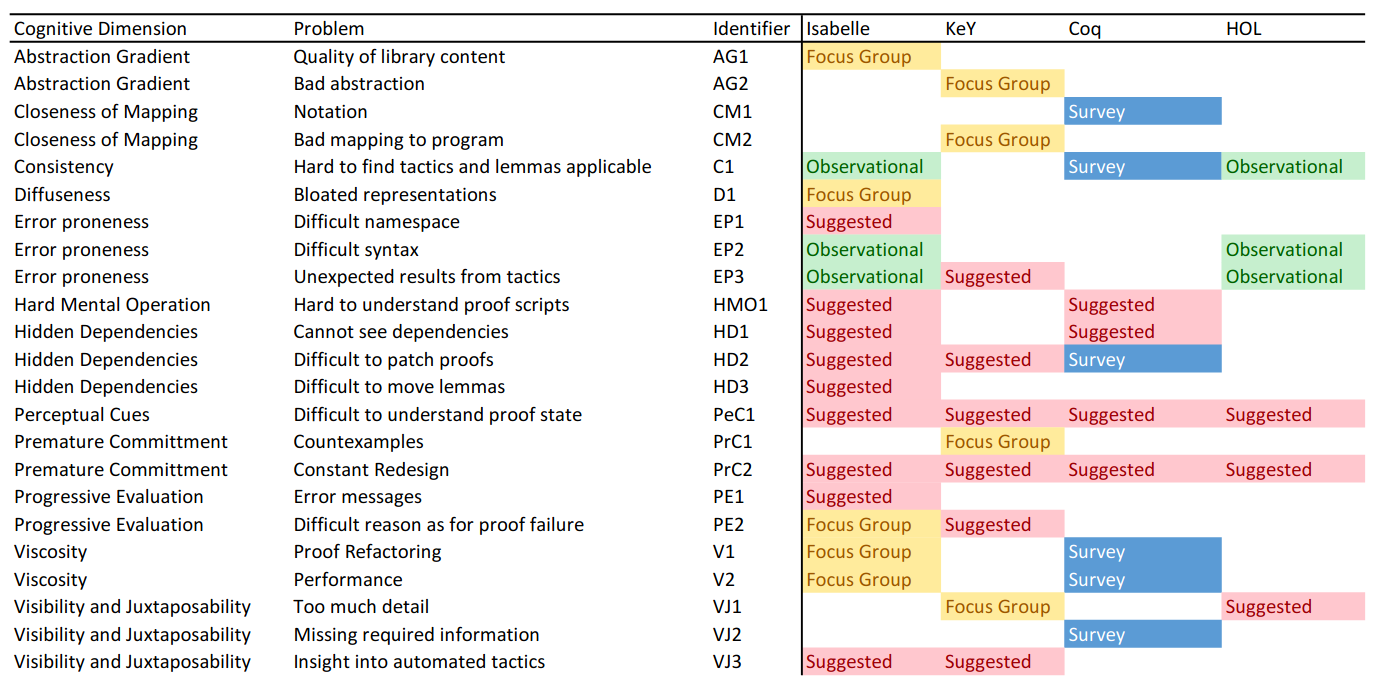
\includegraphics{./Images/MyProblem.png}
\caption{Identified Usability Issues}\label{fig:usability_issues}
}
\end{figure}

This analysis finds that although many issues were identified, there is
very little empirical research on these problems. This is probably due
to the difficulty in recruiting expert participants to these studies,
and the small size of the field.

An empirical analysis of all of these problems is well and truly outside
the scope of this thesis. The task at hand is to now select problems
that can be addressed.

The first thing to consider is that we are creating a living review.
Many of the usability issues that arose have a strong human component.
For instance, ``Hard to predict the results of tactics'' would be very
difficult to evaluate without performing a usability test. If we were to
include a measure within the living review that required the conducting
of a usability test, the usability test would need to be run on a
periodic basis to keep it up to date with the current state of
technology. This is highly undesirable, as such a project would be
extremely time consuming and expensive, and would require a time and
money investment for years after this thesis is published.

To address this, we restrict this thesis to usability issues that can be
determined to exist without the highly expensive intervention of a user.
This leaves the following options:

\begin{itemize}
\tightlist
\item
  Scope of Library
\item
  Math Notation support
\item
  Counterexamples
\item
  Performance
\end{itemize}

All these issues beside performance are within the scope of our living
review. Although creating a living review for ITP performance that
automatically updates is technically feasible, we determined that this
was not a usability problem of interest in comparison to the large
amount of effort and money (setting up a list of standard activities,
setting up of standardised hardware, running programs in test harnesses)
required to include performance the review's scope.

\hypertarget{sec:results}{%
\section{Results}\label{sec:results}}

In this section, we discuss in detail the living review that we have
contributed. This section is only a static snapshot of the review at its
current stage. The full living review is available online and will be
fully up to date. Therefore, it should be noted that the living review
itself contains all the information found in this section and more. If
you wish to view the results as it is up to date, then we invite you to
look through the online widget.

The widget can be explored from the following:
\href{https://samnolan.me/thesis/review.html}{https://samnolan.me/thesis}

The source code for this thesis, the widget, and all the code behind it
are also available on GitHub at
\url{https://github.com/Hazelfire/thesis}. What follows is a snapshot of
the findings in the review.

The following 17 ITPs were included in the review: ACL2
{[}\protect\hyperlink{ref-ACL2}{51}{]}, Agda
{[}\protect\hyperlink{ref-Agda}{64}{]}, Atelier B
{[}\protect\hyperlink{ref-Atelier_B}{25}{]}, Coq
{[}\protect\hyperlink{ref-Coq}{19}{]}, Getfol
{[}\protect\hyperlink{ref-Getfol}{33}{]}, HOL Light
{[}\protect\hyperlink{ref-HOL_Light}{41}{]}, HOL4
{[}\protect\hyperlink{ref-HOL4}{78}{]}, Isabelle
{[}\protect\hyperlink{ref-Isabelle}{68}{]}, JAPE
{[}\protect\hyperlink{ref-JAPE}{21}{]}, LEO-II
{[}\protect\hyperlink{ref-LEO-II}{17}{]}, Lean
{[}\protect\hyperlink{ref-Lean}{61}{]}, Metamath
{[}\protect\hyperlink{ref-Metamath}{65}{]}, Mizar
{[}\protect\hyperlink{ref-Mizar}{34}{]}, PVS
{[}\protect\hyperlink{ref-PVS}{73}{]}, RedPRL
{[}\protect\hyperlink{ref-RedPRL}{5}{]}, Twelf
{[}\protect\hyperlink{ref-Twelf}{69}{]}, and Z/EVES
{[}\protect\hyperlink{ref-Zux2fEVES}{74}{]}.

The results are split into three sections. In
Section~\ref{sec:math_libraries}, results about the state and scope of
mathematical libraries of ITPs are discussed. In
Section~\ref{sec:counterexamples} results about the support of
Counterexample generators are covered. Finally, in
Section~\ref{sec:math_notation} and results about mathematical notation
support are covered.

\hypertarget{sec:math_libraries}{%
\subsection{Mathematical Libraries}\label{sec:math_libraries}}

This section details results about the distribution of mathematical
topics currently covered by ITPs, as of 28 October 2021. All findings,
including the dataset of classified modules, can be viewed and
downloaded in the up to date form by viewing the review online.

The methodology for this section has been laid out in
Section~\ref{sec:scope_of_library_meth}.

\hypertarget{step-1-identifying-libraries}{%
\subsubsection{Step 1: Identifying
Libraries}\label{step-1-identifying-libraries}}

This section corresponds to the section laid out in
Section~\ref{sec:identifying_math_lib_meth}

13 mathematical libraries were covered in this analysis. They are
detailed in Table~\ref{tbl:libraries}.

Twelf was excluded due to not proving any mathematical theorems within
its library, failing IC1.

Getfol and RedPRL failed to meet IC2, in having small libraries with
only 1372 and 2680 lines of proof code respectively.

LEO-II or Z/EVES do not have standard libraries.

\hypertarget{step-2-collecting-modules}{%
\subsubsection{Step 2: Collecting
modules}\label{step-2-collecting-modules}}

As per our methodology, we must now chose what we mean by a module for
comparison. What we chose as a module is listed in
Table~\ref{tbl:libraries} for each ITP.

\renewcommand\arraystretch{1.3}

\hypertarget{tbl:libraries}{}
\begin{longtable}[]{@{}
  >{\raggedright\arraybackslash}p{(\columnwidth - 6\tabcolsep) * \real{0.10}}
  >{\raggedright\arraybackslash}p{(\columnwidth - 6\tabcolsep) * \real{0.26}}
  >{\raggedright\arraybackslash}p{(\columnwidth - 6\tabcolsep) * \real{0.31}}
  >{\raggedright\arraybackslash}p{(\columnwidth - 6\tabcolsep) * \real{0.34}}@{}}
\caption{\label{tbl:libraries}Libraries covered in the living
review}\tabularnewline
\toprule
\begin{minipage}[b]{\linewidth}\raggedright
Name
\end{minipage} & \begin{minipage}[b]{\linewidth}\raggedright
Library
\end{minipage} & \begin{minipage}[b]{\linewidth}\raggedright
Type
\end{minipage} & \begin{minipage}[b]{\linewidth}\raggedright
Module Definition
\end{minipage} \\
\midrule
\endfirsthead
\toprule
\begin{minipage}[b]{\linewidth}\raggedright
Name
\end{minipage} & \begin{minipage}[b]{\linewidth}\raggedright
Library
\end{minipage} & \begin{minipage}[b]{\linewidth}\raggedright
Type
\end{minipage} & \begin{minipage}[b]{\linewidth}\raggedright
Module Definition
\end{minipage} \\
\midrule
\endhead
ACL2 & \href{https://github.com/acl2/acl2/tree/master/books}{Community
Books} & packages & a community book, such as acl2ls or
data-structures \\
Agda &
\href{https://wiki.portal.chalmers.se/agda/Main/Libraries}{Community
Libraries} & packages & a submission such as AoPA or DTGP \\
Agda & \href{https://github.com/agda/agda-stdlib}{Standard Library} &
small & a top level module, such as Data or Algebra \\
Coq & \href{https://coq.inria.fr/library/index.html}{Standard Library} &
small & a top level module, such as Init or Arith \\
Coq & \href{https://coq.inria.fr/opam/www/}{Packages} & packages & a
package \\
HOL Light & \href{https://github.com/jrh13/hol-light}{HOL Light Library}
& large & a second level module, such as Library/analysis.ml or
Multivariate/clifford.ml \\
HOL4 &
\href{https://github.com/HOL-Theorem-Prover/HOL/tree/develop/src}{HOL4
Library} & small & a top level module, such as bool or topology \\
Isabelle & \href{https://isabelle.in.tum.de/dist/library/}{Core
Libraries} & large & a session, such as HOL/HOL-Algebra \\
Isabelle & \href{https://www.isa-afp.org/}{Archive of Formal Proofs} &
packages & a submission \\
Lean &
\href{https://leanprover-community.github.io/mathlib-overview.html}{Lean
Mathematical Library} & large & a second level module, such as
algebra.algebra or probability.distribution \\
Metamath & \href{http://us.metamath.org/mpeuni/mmset.html}{Metamath
Library} & small & a "part", such as "ZF SET THEORY", or one of the
smaller theories, such as "Higher Order Logic" \\
Mizar & \href{http://www.mizar.org/library/}{Mizar Mathematical Library}
& package & a submission, such as abian of aff\_2 \\
PVS & \href{https://github.com/nasa/pvslib}{NASA PVS Library of Formal
Developments} & packages & a module, such as algebra or analysis \\
\bottomrule
\end{longtable}

Justifications for each module size are given below:

\textbf{ACL2 - Community Books:} A community book is a community
contributed module for ACL2. They are stored within the ACL2 source
tree. One community book was seen as the natural mapping to a module.
Community books however cover a range of topics, not all mathematical.

\textbf{Agda - Community Libraries:} The collection of Agda community
libraries are a very informal list of contributions found on the Agda
Wiki, where users can add their contribution to a simple dot point list
on the page. A single item per module was seen as a natural mapping to a
module.

\textbf{Agda - Standard Library:} Agda's "standard library" is an
unofficial standard library for Agda. Although Agda's library was chosen
to be small, it is definitely on the larger side of small. Agda was
chosen to be a small library because splitting the library by any level
lower than the top level would result in a very large amount of tiny
modules, such as many modules containing less than 100 lines of code
each defining a single data type. As of such, having this library be
considered small better represents the size of it, even if it may
underrepresent it's scope by defining larger modules.

\textbf{Coq - Standard Library:} Coq's library is small, and does not
have many items that would be interesting to a mathematician. It
resembles that of a standard programming library, containing basic
definitions of data types and a few properties about basic algebraic
structures such as rings. However, it does have some modules of interest
as a mathematician, so we considered it a small library.

\textbf{Coq - Packages:} Coq's package management system has a wide
vaiety of packages. A package in Coq's package management system is the
natural way of dividing up the packages into modules. However, some
packages are very large and cover a large amount of topics.

\textbf{HOL Light - HOL Light Library:} HOL Light's library has a wide
range of support for different areas of mathematics. A module was chosen
to be a single file as the files in HOL Light cover a very large amount
of topics, and are frequently above 1500 lines.

\textbf{HOL4 - HOL4 Library:} HOL4's libary has a large amount of
variance in module size. With some top level modules being quite large
such as probability, whereas others are much smaller than a standard
module such as topology. A small library size was chosen as it better
approximated "package sized" modules. However, the library is
nevertheless expansive on some topics.

\textbf{Isabelle - Core Libraries:} Isabelle's library sorts itself into
three levels, with several different libraries being on the first level,
sessions being on the second, and individual theory files being on the
third. Most of the modules come from the HOL library, and have support
for many constructs that would be useful for a mathematician. As of
such, individual sessions were chosen as the definition of a module.
However, the sizes of Isabelle's modules varies widely, from some being
much larger than the size we were aiming for and others being much
smaller.

\textbf{Isabelle - Archive of Formal Proofs:} A submission is the
natural way of dividing up the Archive of Formal Proofs. A submission is
in essense very similar to a package.

\textbf{Lean - Lean Mathematical Library:} Lean's library is possibly
the biggest library in this analysis. This library was therefore
considered large, as it best approximates a "packaged size" module.
However, the sizes of these modules are relatively inconsistent, with
some modules being much larger and others being much smaller.

\textbf{Metamath - Metamath Library:} One "Part" has enough metamath
code to make up about a "package sized" module. It should be noted that
there was a minor exception to the standard methodology with Metamath.
Metamath has several libraries, where the main library was split up as
if it was a small library. However, there are alternative libraries that
were so small that each one contributes about the size of a single
module. As of such, these were included as single modules.

\textbf{Mizar - Mizar Mathematical Library:} although Mizar's library is
called the "Mizar Mathematical Library". The library operates more like
a repository of community contributions, and as of such the natural
transformation is for one contribution to be a module. This however, is
slightly misrepresentative, as a community contribution in Mizar is much
smaller than the target of 1500 "package sized" module.

\textbf{PVS - NASA PVS Library of Formal Developments:} PVS's library
has a collection of modules which formed the natural mapping to modules.
Many of these are relevant more to computer science than mathametics.

\hypertarget{step-3-classifying-modules}{%
\subsubsection{Step 3: Classifying
modules}\label{step-3-classifying-modules}}

From these libraries, 5581 math modules were collected libraries. From
these modules, 5527 were manually verified and classified into an
appropriate MSC2020 classification or excluded. The sizes of these
libraries are displayed in Figure~\ref{fig:total_itp_modules}.

\begin{sidewaysfigure}
    \centering
    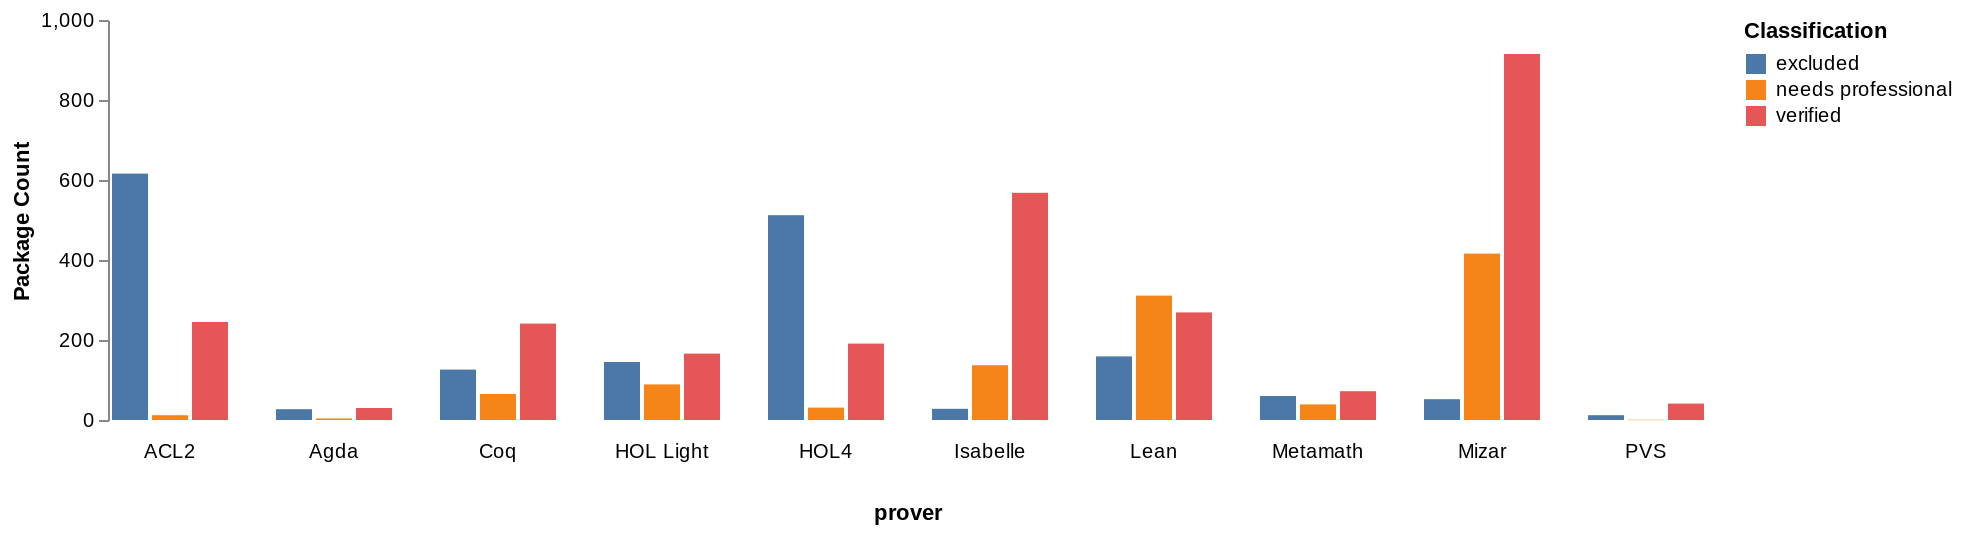
\includegraphics{./Images/ITPTotal.png}
    \caption{Amount of modules found in each ITP}
    \label{fig:total_itp_modules}
\end{sidewaysfigure}

This therefore represents an incomplete classification of the packages.
The main source of incompleteness came from a lack of understand of the
module's purposes by the author. Nevertheless, most of the modules were
verified, and we can get an insight to the field of ITPs from it.

In descending order of the amount of total mathematical modules, a
description of the classification for each ITP is given:

\textbf{Mizar - Mizar Mathematical Library}: Has a total of 1383
modules. Of these modules, 52 module were excluded. Including 16 module
were excluded for being a utility (EC1). 915 modules were verified into
categories and 416 require a professional mathematician to properly
categorise.

\textbf{ACL2 - Community Books}: Has a total of 873 modules. Of these
modules, 616 module were excluded. Including 448 module were excluded
for being a utility (EC1), 53 module were excluded for being only
documentation (EC3), and 26 module were excluded for being deprecated
(EC4). 245 modules were verified into categories and 12 require a
professional mathematician to properly categorise.

\textbf{Lean - Lean Mathematical Library}: Has a total of 739 modules.
Of these modules, 159 module were excluded. Including 150 module were
excluded for being a utility (EC1), one module was excluded for being
only documentation (EC3), and 6 module were excluded for being
deprecated (EC4). 269 modules were verified into categories and 311
require a professional mathematician to properly categorise.

\textbf{HOL4 - HOL4 Library}: Has a total of 734 modules. Of these
modules, 512 module were excluded. Including 294 module were excluded
for being a utility (EC1) and one module was excluded for being only
documentation (EC3). 191 modules were verified into categories and 31
require a professional mathematician to properly categorise.

\textbf{Isabelle - Archive of Formal Proofs}: Has a total of 611
modules. Of these modules, 3 module were excluded. Including 3 module
were excluded for being a utility (EC1). 495 modules were verified into
categories and 113 require a professional mathematician to properly
categorise.

\textbf{HOL Light - HOL Light Library}: Has a total of 400 modules. Of
these modules, 145 module were excluded. Including 71 module were
excluded for being a utility (EC1) and 25 module were excluded for being
only documentation (EC3). 166 modules were verified into categories and
89 require a professional mathematician to properly categorise.

\textbf{Coq - Packages}: Has a total of 396 modules. Of these modules,
119 module were excluded. Including 114 module were excluded for being a
utility (EC1), one module was excluded for being only documentation
(EC3), and 3 module were excluded for being deprecated (EC4). 214
modules were verified into categories and 63 require a professional
mathematician to properly categorise.

\textbf{Metamath - Metamath Library}: Has a total of 171 modules. Of
these modules, 60 module were excluded. Including 42 module were
excluded for being a utility (EC1), 2 module were excluded for being
only documentation (EC3), and 16 module were excluded for being
deprecated (EC4). 72 modules were verified into categories and 39
require a professional mathematician to properly categorise.

\textbf{Isabelle - Core Libraries}: Has a total of 123 modules. Of these
modules, 25 module were excluded. Including one module was excluded for
being a utility (EC1) and 18 module were excluded for being only
documentation (EC3). The classification was not complete, as there was 1
unclassified modules. 73 modules were verified into categories and 24
require a professional mathematician to properly categorise.

\textbf{PVS - NASA PVS Library of Formal Developments}: Has a total of
54 modules. Of these modules, 12 module were excluded. Including 11
module were excluded for being a utility (EC1) and one module was
excluded for being only documentation (EC3). 41 modules were verified
into categories and 1 require a professional mathematician to properly
categorise.

\textbf{Agda - Community Libraries}: Has a total of 43 modules. Of these
modules, 19 module were excluded. Including 13 module were excluded for
being a utility (EC1) and 2 module were excluded for being only
documentation (EC3). 21 modules were verified into categories and 3
require a professional mathematician to properly categorise.

\textbf{Coq - Standard Library}: Has a total of 36 modules. Of these
modules, 7 module were excluded. Including 7 module were excluded for
being a utility (EC1). 27 modules were verified into categories and 2
require a professional mathematician to properly categorise.

\textbf{Agda - Standard Library}: Has a total of 18 modules. Of these
modules, 8 module were excluded. Including 8 module were excluded for
being a utility (EC1). 9 modules were verified into categories and 1
require a professional mathematician to properly categorise.

It was found that some libraries were clear outliers in mathematical
scope covered. Those libraries were Coq, HOL Light, Isabelle, Lean, and
Mizar. It would be difficult to justify use of other theorem provers as
a mathematician getting into the field.

HOL4, HOL Light and ACL2 have a lot of excluded module due to having
many utilities available for the user. For instance, in HOL Light

To recall, a package starts as unclassified, then it's automatically
classified if there's any category system available and becomes
unverified. Then the package is examined do determine what category it
belongs to and then it is either excluded or verified.

The largest library by modules was Mizar with 1383 modules. This
however, as noted above, may not fully representative. Mizar also has
the largest amount of unclassified modules, as Mizar's Mathematical
Library doesn't have any categorization or structure to modules.

Coq, HOL Light had a large amount of excluded modules for being
utilities. Most of HOL4 exclusions were from no documentation.

\begin{sidewaysfigure}
    \centering
    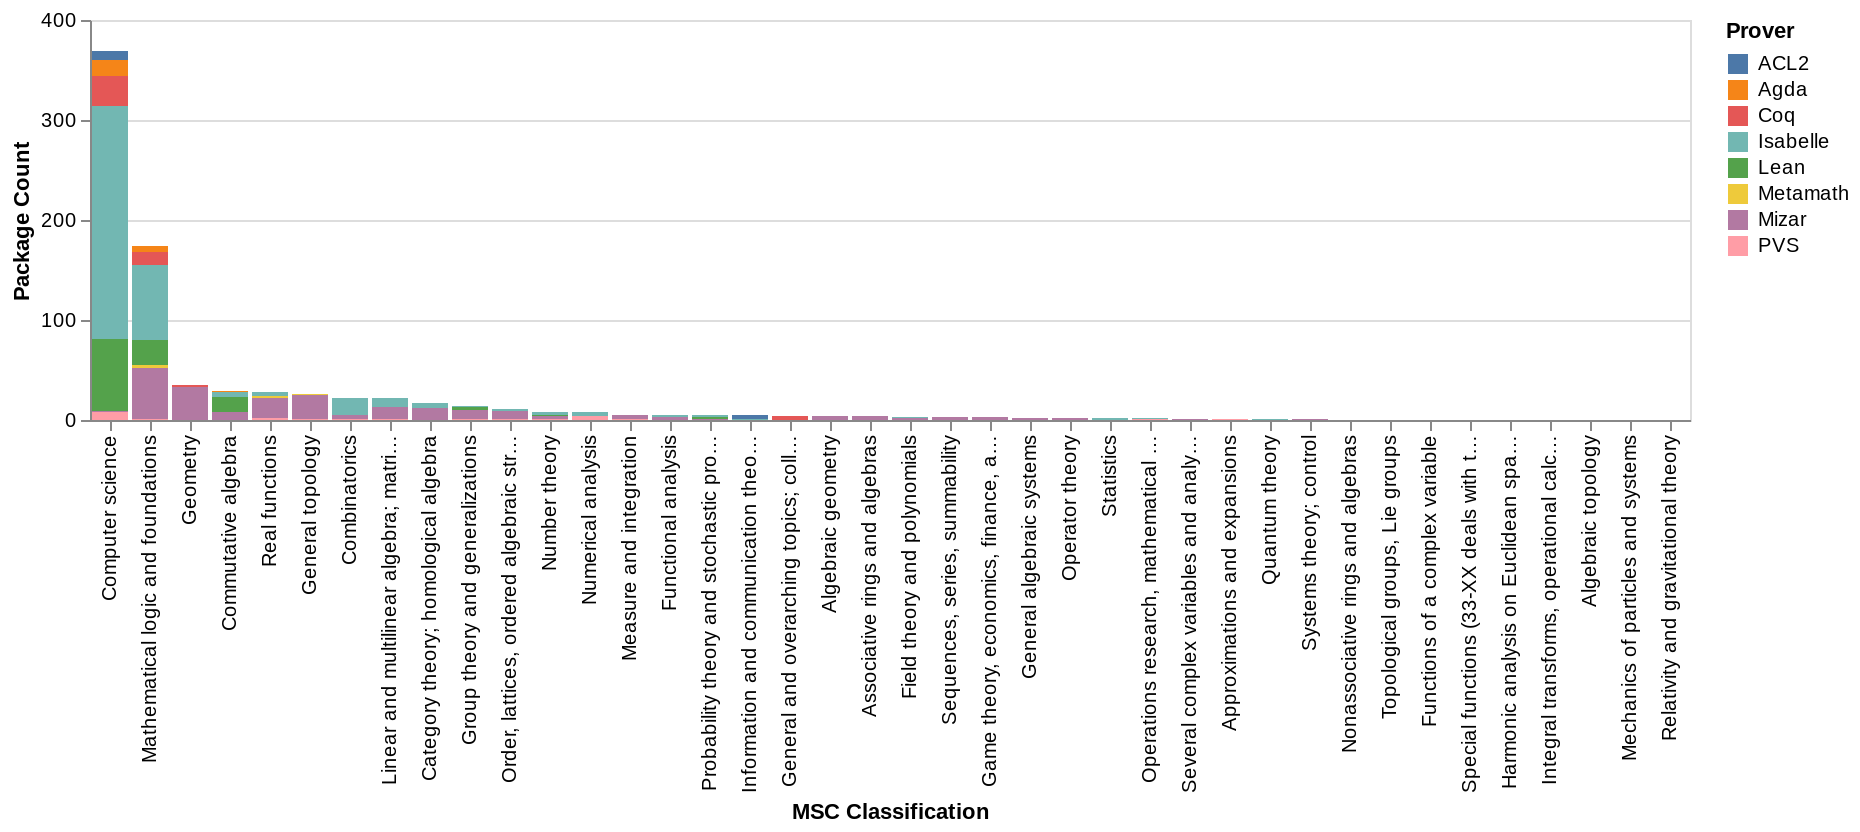
\includegraphics{./Images/MathClassification.png}
    \caption{Math Package classifications, as of 28 October 2021}
    \label{fig:math_classifications}
\end{sidewaysfigure}

The chart in Figure~\ref{fig:math_classifications} shows which verified
top level MSC Classifications these modules were sorted into as of 28
October 2021. Each column represents a top level classification of a
mathematical topic from MSC2020 (as described in
Section~\ref{sec:scope_of_library_meth}, sorted by by the amount of
total modules in each classification. Each colour represents modules
from a different ITP.

This chart was created using Vega-Lite
{[}\protect\hyperlink{ref-Vega-Lite}{75}{]} a chart visualisation
framework. It is reproduced in the living review where it is fully up to
date and is further interactive, showing the exact modules counts when
hovering with a mouse.

The chart represents the mathematical scope of each of the libraries. If
a particular field has more modules, it represents a larger availability
of prior work to build upon when developing new proofs, therefore less
working from the ground up.

\textbf{Computer science (68-XX)}: Had a total of 978 modules. The ITPs
with the most packages in this category were \emph{Isabelle} with 323
modules, \emph{HOL4} with 158 modules, and \emph{Coq} with 146 modules.
The most popular second level MSC classifications were \emph{Theory of
data} (68Pxx) with 320 modules, \emph{Theory of computing} (68Qxx) with
252 modules, and \emph{Theory of software} (68Nxx) with 151 modules, and
finally, the most popular third level classifications were \emph{Data
structures} (68P05) with 269 modules, \emph{Specification and
verification (program logics, model checking, etc.) } (68Q60) with 102
modules, and \emph{Theory of programming languages} (68N15) with 51
modules.

\textbf{Mathematical logic and foundations (03-XX)}: Had a total of 548
modules. The ITPs with the most packages in this category were
\emph{Mizar} with 188 modules, \emph{Isabelle} with 113 modules, and
\emph{Coq} with 53 modules. The most popular second level MSC
classifications were \emph{Set theory} (03Exx) with 183 modules,
\emph{General logic} (03Bxx) with 180 modules, and \emph{Proof theory
and constructive mathematics} (03Fxx) with 56 modules, and finally, the
most popular third level classifications were \emph{Set theory} (03Exx)
with 62 modules, \emph{Classical first-order logic} (03B10) with 50
modules, and \emph{Ordinal and cardinal numbers} (03E10) with 32
modules.

\textbf{Number theory (11-XX)}: Had a total of 209 modules. The ITPs
with the most packages in this category were \emph{Mizar} with 63
modules, \emph{HOL Light} with 46 modules, and \emph{Isabelle} with 38
modules. The most popular second level MSC classifications were
\emph{Elementary number theory } (11Axx) with 72 modules and
\emph{Sequences and sets} (11Bxx) with 19 modules, and finally, the most
popular third level classifications were \emph{Number theory} (11-XX)
with 34 modules, \emph{Factorization; primality} (11A51) with 21
modules, and \emph{Congruences; primitive roots; residue systems}
(11A07) with 17 modules.

\textbf{Real functions (26-XX)}: Had a total of 186 modules. The ITPs
with the most packages in this category were \emph{Mizar} with 89
modules, \emph{HOL Light} with 36 modules, and \emph{Metamath} with 21
modules. The most popular second level MSC classifications were
\emph{Functions of one variable} (26Axx) with 90 modules and
\emph{Functions of several variables} (26Bxx) with 34 modules, and
finally, the most popular third level classifications were
\emph{Functions of several variables} (26Bxx) with 30 modules,
\emph{Real functions} (26-XX) with 29 modules, and \emph{Integrals of
Riemann, Stieltjes and Lebesgue type } (26A42) with 21 modules.

\textbf{General topology (54-XX)}: Had a total of 185 modules. The ITPs
with the most packages in this category were \emph{Mizar} with 121
modules, \emph{Lean} with 46 modules, and \emph{HOL Light} with 6
modules. The most popular second level MSC classifications were
\emph{Topological spaces with richer structures} (54Exx) with 24 modules
and \emph{Fairly general properties of topological spaces} (54Dxx) with
20 modules, and finally, the most popular third level classifications
were \emph{General topology } (54-XX) with 114 modules, \emph{Metric
spaces, metrizability} (54E35) with 14 modules, and \emph{Compactness}
(54D30) with 7 modules.

\textbf{Order, lattices, ordered algebraic structures (06-XX)}: Had a
total of 179 modules. The ITPs with the most packages in this category
were \emph{Mizar} with 101 modules, \emph{Lean} with 50 modules, and
\emph{Isabelle} with 12 modules. The most popular second level MSC
classifications were \emph{Lattices } (06Bxx) with 60 modules and
\emph{Ordered structures} (06Fxx) with 19 modules, and finally, the most
popular third level classifications were \emph{Order, lattices, ordered
algebraic structures} (06-XX) with 67 modules, \emph{Continuous lattices
and posets, applications } (06B35) with 25 modules, and \emph{Lattices }
(06Bxx) with 21 modules.

\textbf{Combinatorics (05-XX)}: Had a total of 147 modules. The ITPs
with the most packages in this category were \emph{Isabelle} with 54
modules, \emph{Mizar} with 46 modules, and \emph{HOL Light} with 18
modules. The most popular second level MSC classifications were
\emph{Graph theory } (05Cxx) with 93 modules and \emph{Enumerative
combinatorics } (05Axx) with 31 modules, and finally, the most popular
third level classifications were \emph{Graph theory } (05Cxx) with 21
modules, \emph{Permutations, words, matrices} (05A05) with 15 modules,
and \emph{Trees} (05C05) with 15 modules.

\textbf{Category theory; homological algebra (18-XX)}: Had a total of
137 modules. The ITPs with the most packages in this category were
\emph{Lean} with 70 modules, \emph{Mizar} with 41 modules, and
\emph{Isabelle} with 12 modules. The most popular second level MSC
classifications were \emph{General theory of categories and functors}
(18Axx) with 38 modules and \emph{Categories and theories} (18Cxx) with
9 modules, and finally, the most popular third level classifications
were \emph{Category theory; homological algebra } (18-XX) with 59
modules, \emph{General theory of categories and functors} (18Axx) with 9
modules, and \emph{Monads (= standard construction, triple or triad),
algebras for monads, homology and derived functors for monads } (18C15)
with 8 modules.

\textbf{Commutative algebra (13-XX)}: Had a total of 135 modules. The
ITPs with the most packages in this category were \emph{Lean} with 71
modules, \emph{Mizar} with 42 modules, and \emph{Isabelle} with 8
modules. The most popular second level MSC classifications were
\emph{Theory of modules and ideals in commutative rings} (13Cxx) with 22
modules and \emph{General commutative ring theory} (13Axx) with 18
modules, and finally, the most popular third level classifications were
\emph{Commutative algebra} (13-XX) with 54 modules, \emph{Polynomials
over commutative rings } (13B25) with 12 modules, and \emph{Structure,
classification theorems for modules and ideals in commutative rings}
(13C05) with 12 modules.

\textbf{Geometry (51-XX)}: Had a total of 135 modules. The ITPs with the
most packages in this category were \emph{Mizar} with 79 modules,
\emph{HOL Light} with 25 modules, and \emph{Isabelle} with 14 modules.
The most popular second level MSC classifications were \emph{Real and
complex geometry} (51Mxx) with 42 modules and \emph{Analytic and
descriptive geometry} (51Nxx) with 24 modules, and finally, the most
popular third level classifications were \emph{Elementary problems in
Euclidean geometries} (51M04) with 35 modules and \emph{Geometry }
(51-XX) with 17 modules.

\textbf{Linear and multilinear algebra; matrix theory (15-XX)}: Had a
total of 118 modules. The ITPs with the most packages in this category
were \emph{Mizar} with 49 modules, \emph{Lean} with 45 modules, and
\emph{Isabelle} with 14 modules. The most popular second level MSC
classifications were \emph{Basic linear algebra} (15Axx) with 69 modules
and \emph{Special matrices} (15Bxx) with 9 modules, and finally, the
most popular third level classifications were \emph{Linear and
multilinear algebra; matrix theory} (15-XX) with 40 modules,
\emph{Vector spaces, linear dependence, rank, lineability} (15A03) with
20 modules, and \emph{Determinants, permanents, traces, other special
matrix functions } (15A15) with 7 modules.

\textbf{Group theory and generalizations (20-XX)}: Had a total of 102
modules. The ITPs with the most packages in this category were
\emph{Lean} with 39 modules, \emph{Mizar} with 39 modules, and
\emph{Isabelle} with 8 modules. The most popular second level MSC
classifications were \emph{Abelian groups} (20Kxx) with 14 modules and
\emph{Foundations} (20Axx) with 8 modules, and finally, the most popular
third level classifications were \emph{Group theory and generalizations}
(20-XX) with 51 modules, \emph{Axiomatics and elementary properties of
groups} (20A05) with 8 modules, and \emph{Abelian groups} (20Kxx) with 6
modules.

\hypertarget{sec:counterexamples}{%
\subsection{Counterexample generators}\label{sec:counterexamples}}

Counterexample generators have been suggested to be beneficial in
helping users understand the proof state they they were in
{[}\protect\hyperlink{ref-beckert_usability_2015}{15}{]}.

This living review covers 3 counter example generators. These
counterexamples generators were;

\textbf{Nitpick} {[}\protect\hyperlink{ref-Nitpick}{20}{]}: Nitpick is a
counterexample generator for Isabelle/HOL. It is fundementally a model
finder and works by using the relational model finder KodKod
{[}\protect\hyperlink{ref-KodKod}{81}{]} as a backend. Model finders are
akin to SAT solvers, in that they work by attempting to find a
collection of values that satisfy a given statement. Nitpick uses model
finders in order to find possible counterexamples. Nitpick also
outperforms QuickCheck. It has support for Isabelle.

\textbf{Nunchaku} {[}\protect\hyperlink{ref-NanchakuCoq}{26},
\protect\hyperlink{ref-NanchakuLean}{67}{]}: Nunchaku is a
counterexample generator intended to be the successor of Nitpick. One of
its main advantages over Nitpick is that it's designed to work with
multiple different frontends (ITPs), as well as different backends, such
as CVC4 {[}\protect\hyperlink{ref-CVC4}{11}{]}. It has support for
Isabelle, Coq, and Lean.

\textbf{QuickCheck} {[}\protect\hyperlink{ref-QuickCheckIsabelle}{23},
\protect\hyperlink{ref-QuickChick}{28},
\protect\hyperlink{ref-QuickCheckAgda}{29},
\protect\hyperlink{ref-DoubleCheck}{31},
\protect\hyperlink{ref-PVSQuickCheck}{66}{]}: QuickCheck is a type of
property based random testing tool. It's not a particular piece of
software but has many implementations in many languages. It works by
specifying a property that you want to test about a system, and
QuickCheck attempts to falsify that the property holds by giving
attempting checking to see if there are counterexamples. Often
QuickCheck is simply used for sotware testing, as it is in Haskell
{[}\protect\hyperlink{ref-QuickCheckHaskell}{24}{]}. However, in the
context of theorem provers, it can be used to find counterexamples to
statement you might wish to prove. It has support for Agda, Isabelle,
PVS, Coq, and ACL2.

This leaves Atelier B, Getfol, HOL Light, HOL4, JAPE, LEO-II, Metamath,
Mizar, RedPRL, Twelf, and Z/EVES not having counter example generators.

\hypertarget{sec:math_notation}{%
\subsection{Math Notation in libraries}\label{sec:math_notation}}

Support of mathematical notation was suggested
{[}\protect\hyperlink{ref-zacchiroli_user_2007}{87}{]}.

The ITPs that use math notation include:

\textbf{Agda}: Agda has support for Unicode characters. And uses Unicode
characters in its math library. This often requires special editor
integrations to input the Unicode characters. Figure~\ref{fig:agda_code}
Shows an example of Agda code

\begin{figure}
\hypertarget{fig:agda_code}{%
\centering
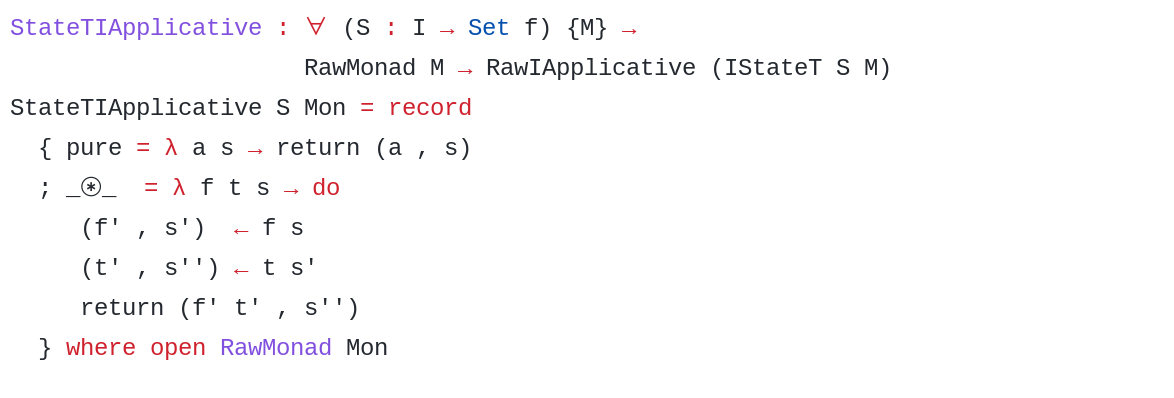
\includegraphics{Images/Notation/Agda.png}
\caption{Agda source code example, from standard library,
Category.Monad.State}\label{fig:agda_code}
}
\end{figure}

\textbf{Isabelle}: Isabelle uses LaTeX math commands to represent math
notation. This is strong supported within the IDE. The saved plaintext
is chown in Figure~\ref{fig:isabelle_raw}.

\begin{figure}
\hypertarget{fig:isabelle_raw}{%
\centering
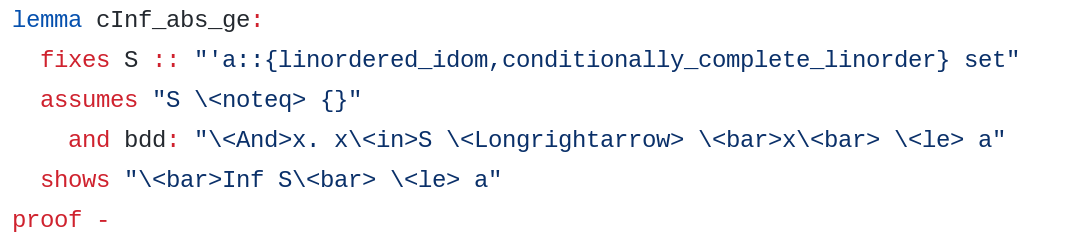
\includegraphics{Images/Notation/IsabelleRaw.png}
\caption{Isabelle source code raw, from core libraries,
HOL/Archimedian\_Field.thy}\label{fig:isabelle_raw}
}
\end{figure}

Whereas the rendered version shown in
Figure~\ref{fig:isabelle_rendered}.

\begin{figure}
\hypertarget{fig:isabelle_rendered}{%
\centering
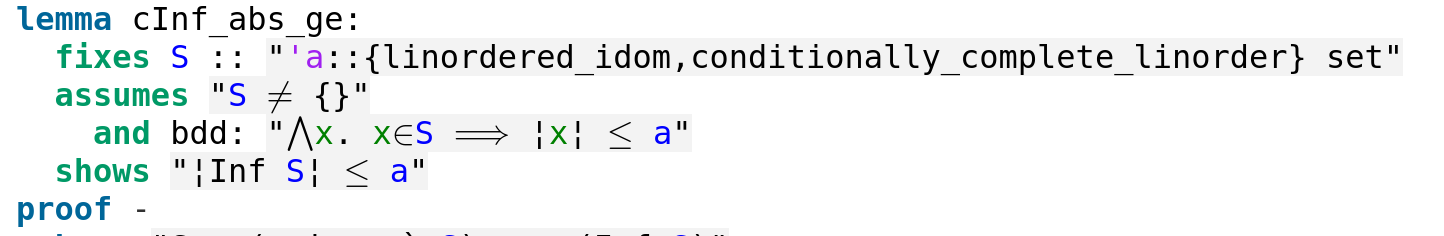
\includegraphics{Images/Notation/IsabelleRender.png}
\caption{Isabelle source code rendered, from core libraries,
HOL/Archimedian\_Field.thy}\label{fig:isabelle_rendered}
}
\end{figure}

\textbf{Lean}: Lean has allows representing math notation using Unicode.
As shown in Figure~\ref{fig:lean_example}.

\begin{figure}
\hypertarget{fig:lean_example}{%
\centering
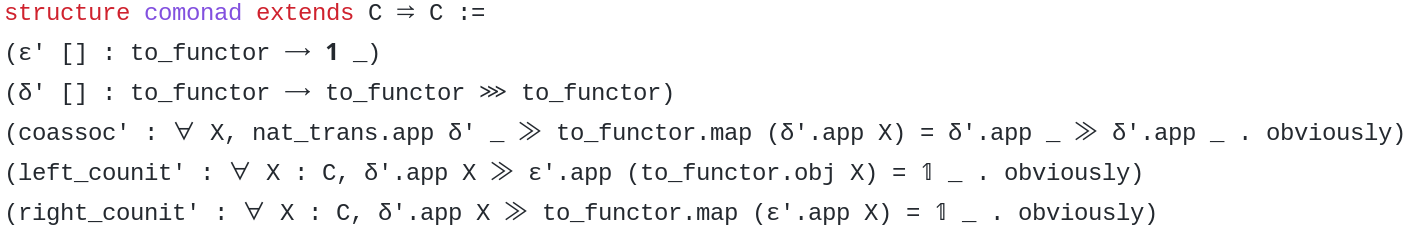
\includegraphics{Images/Notation/LeanUnicode.png}
\caption{Lean source code rendered, from mathlib,
category.monad.basic}\label{fig:lean_example}
}
\end{figure}

\textbf{Z/EVES}: Z/EVES uses LaTeX commands to prove propositions. The
interface, much like Isabelle, allows the user to press buttons on the
interface to input notation. As shown in Figure~\ref{fig:zeves_example}.

\begin{figure}
\hypertarget{fig:zeves_example}{%
\centering
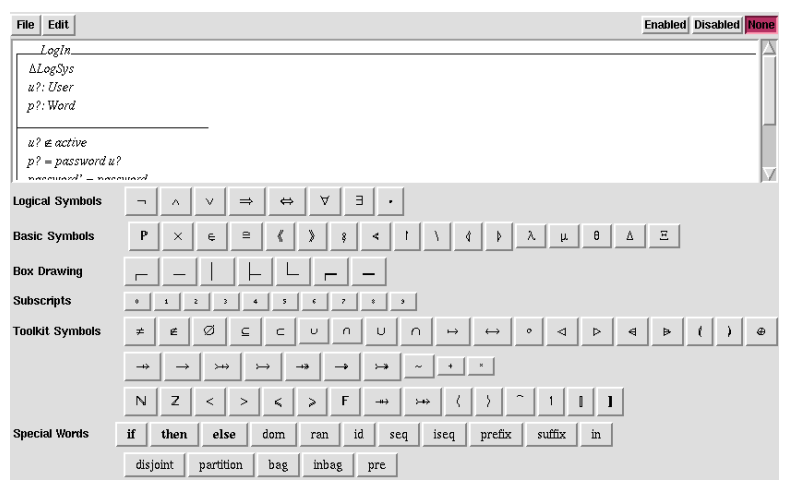
\includegraphics{Images/Notation/Zeves.png}
\caption{Z/EVES notation support}\label{fig:zeves_example}
}
\end{figure}

The ITPs in this study without math notation are ACL2, Atelier B, Coq,
Getfol, HOL Light, HOL4, JAPE, LEO-II, Metamath, Mizar, PVS, RedPRL, and
Twelf. These theorem provers may also be improved with math notation
support.

\textbf{Agda}: Agda has support for unicode characters. And uses unicode
characters in its math library. This often requires special editor
integrations to input the unicode characters..

\textbf{Isabelle}: Isabelle uses LaTeX math commands to represent math
notation. This is strong supported within the IDE.

\textbf{Lean}: Lean has allows representing math notation on LaTeX..

\textbf{Z/EVES}: Z/EVES uses LaTeX commands to prove propositions.

The ITPs in this study without math notation are ACL2, Atelier B, Coq,
Getfol, HOL Light, HOL4, JAPE, LEO-II, Metamath, Mizar, PVS, RedPRL, and
Twelf. These theorem provers may also be improved with math notation
support.

\hypertarget{discussion}{%
\section{Discussion}\label{discussion}}

We evaluate this review by comparing it to other literature reviews, and
other living reviews.

There are not a large amount of literature reviews in the space of ITPs,
but we shall first compare it to the literature review the data was
based on.

It should first stand to say that this is the first living review on
ITPs. As of such, this review already has many benefits over the current
literature.

The clear improvement is this is the only review on ITPs that
automatically updates to reflect the current state of the art. This
means it can be referred back to at any time, and even used to track
progress on efforts, such as formalizing mathematics.

Due to the availability of web technologies and interactivity, the
living review is also much more accessible than a paper one. It allows
readers to compare features of ITPs without scouring through large
amounts of text or needing to pay large amounts of money to find them.
The use of interactive tables and multiple pages in our review mean that
the user can extract the knowledge that they are interested in without
difficulty.

These benefits of the fact that it is living are great, but even without
considering them, this review does build on past reviews.

This is the first review to ever classify the completed scope of ITPs.
The classification helps people become aware of package in their field.

A good place to start in comparison is the literature review we base
some of our data on {[}\protect\hyperlink{ref-nawaz_survey_2019}{63}{]}.
This review covers Theorem Provers in Formal Methods and what features
they have. This literature review covers both Automatic Theorem Provers
and Interactive Theorem Provers. For the sake of ITPs, the review has
the scope of discovering what features each ITP has. This living review
includes all of the features and compares them, but also explains what
these features mean for a particular provers, allowing newcomers to
better understand the field. The living review also offers the benefits
of being able to check the differences between mathematical libraries.
This, in the domain of ITPs, therefore contains a superset of the
knowledge in this one. This is however expected, as we used this review
as a basis for our one.

Other literature reviews include a survey on the field of Interactive
Theorem Proving {[}\protect\hyperlink{ref-a_survey_of_itp}{56}{]}. This
review covers a brief history of ITPs, and a discussion of different
calculi present in ITPs. This survey has a larger scope in terms of
history, and detailed discussions of types of calculus and achievements.
It however, is not systematic, and more represents an introduction to
the field of ITPs, and may not be suitable for those currently in the
field to understand the current state of the art. Furthermore, this
review is difficult to understand without a strong knowledge of logic.

Finally, John Harrison completed a review of the history of ITPs
{[}\protect\hyperlink{ref-history_of_itps}{42}{]}. As the title
suggests, this review covers the history of ITPs, which is again outside
the scope of this living review. This review is comprehensive in
covering the development of ITPs up until 2014. However, at 7 years, it
is currently out of date.

\hypertarget{limitations-with-current-work}{%
\subsection{Limitations with current
work}\label{limitations-with-current-work}}

As much as this work does make progress on the current state of the
field, it is not without limitations. This section covers possible
limitations on this work, or items that were deemed out of scope but
would be helpful.

One limitation of this work is that although it does represent a review
of the field, the review would likely not be suitable as an
introduction. Often, reviews allow users unfamiliar with a field to
introduce themselves and better understand the topic so that they can
make direct work. This review does not do this, and instead tracks the
progress of the field, and may be more suitable to people within it.

A second limitation is that the author is not a mathematician by
training, and there were a large number of modules that may require help
from a professional mathematician to fully classify. Further, this
review may contain errors in it due to the author not having training in
the field. Living reviews can update over time however, and it is
entirely possible that a mathematician could volunteer their time to
complete the classification, or incorporate ways to suggest changes by

A third limitation is that although this is a living review, it does not
often reference conference papers or journal articles, even though it
possibly could. A more complete living review might include a discussion
of the current trends in research, such as the usability research done
on a particular theorem prover. We chose to exclude this from the
current contribution due to requiring a large amount of manual work to
keep up to date. However, we are convinced that such a review would be
worth the effort in creating.

\hypertarget{future-work}{%
\subsection{Future Work}\label{future-work}}

During this investigation, several avenues of future work became clear.

Firstly, it was identified that the field of ITPs lacks empirical
usability studies. Work in identifying and verifying usability issues
with ITPs would do a good job to fill the gap in the literature. Many of
the issues that arose in this review could be fantastic candidates.

Secondly, due to the nature of a living review, it is entirely possible
to extend the scope over time. For instance, we considered the scope of
libraries, counterexample generators and math provers. One possible
extension of the review would be collecting large projects done in ITPs,
in order to demonstrate their ability and usage in industry settings.
This was outside the scope of this living review, but it could be
updated in the future. This way a user from industry could consider
whether they should invest in ITPs for their software project.

Finally, the author does hope that this may encourage the creation of
more living reviews for other topics. A living review has many
advantages, one of the most prominent being it is a considerably more
accessible way of presenting information in a field, both to
professionals and non professionals.

\hypertarget{summary}{%
\subsection{Summary}\label{summary}}

ITPs are important due to their ability to assure very high levels of
quality in software, which is only needed more as our reliance on
technology only increases. However, ITPs have not yet had a large
industry uptake, and it has been suggested
{[}\protect\hyperlink{ref-kadoda_formal_1997}{49}{]} that usability
issues with the ITPs could be the reason.

Motivated to investigate why a user might find the adoption of ITPs
difficult, we performed a systematic literature review on usability
issues mentioned in literature. We found there was a profound lack of
empirical studies on usability about ITPs, and that there was a large
number of potential usability problems that could be investigated.

From this systematic literature review, we decided to attempt to shed
more light on these usability issues. We did this by creating a living
review of ITPs. The review semi-automatically update periodically to
reflect the current state of the field. This living review was designed
with the intent of being accessible to newcomers, but also to ensure
that it doesn't become invalid years down the track.

In this living review, we examined the usability issues of small
mathematical scopes, lack of counterexample generators and lack of math
notation. We did this by systematically examining math modules created
for ITPs, and classified them to the Mathematical Subject
Classification. This allows readers to compare ITPs by the areas of
mathematics that they cover, helping mathematicians make decisions about
ITPs. Further, it tracks progress towards the formalization of different
sections of mathematics.

We identified that some ITPs are currently better for different topics.
Particularly depending on whether you want are looking to verify
software or prove mathematical theorems. However, even if you wanted to
prove mathematical theorems, different ITPs were better in different
situations depending on the mathematical field.

We also directly examined the ITPs for counterexample generators and
support for math notation, and included this within our living review.

This review will be updated periodically and therefore will remain a
reference for the field.

\hypertarget{bibliography}{%
\section*{Bibliography}\label{bibliography}}
\addcontentsline{toc}{section}{Bibliography}

\hypertarget{refs}{}
\begin{CSLReferences}{0}{0}
\leavevmode\vadjust pre{\hypertarget{ref-Dijkstra}{}}%
\CSLLeftMargin{{[}1{]} }
\CSLRightInline{2008. Shortest paths. \emph{Algorithms and data
structures: The basic toolbox}. Springer Berlin Heidelberg. 191--215.}

\leavevmode\vadjust pre{\hypertarget{ref-HOL_Zero}{}}%
\CSLLeftMargin{{[}2{]} }
\CSLRightInline{Adams, M. 2010. Introducing HOL zero. \emph{Mathematical
software -- ICMS 2010} (Berlin, Heidelberg, 2010), 142--143.}

\leavevmode\vadjust pre{\hypertarget{ref-aitken_interactive_1998}{}}%
\CSLLeftMargin{{[}3{]} }
\CSLRightInline{Aitken, J.S., Gray, P., Melham, T. and Thomas, M. 1998.
Interactive {Theorem} {Proving}: {An} {Empirical} {Study} of {User}
{Activity}. \emph{Journal of Symbolic Computation}. 25, 2 (1998),
263--284.
DOI:https://doi.org/\url{https://doi.org/10.1006/jsco.1997.0175}.}

\leavevmode\vadjust pre{\hypertarget{ref-aitken_analysis_2000}{}}%
\CSLLeftMargin{{[}4{]} }
\CSLRightInline{Aitken, S. and Melham, T. 2000. An analysis of errors in
interactive proof attempts. \emph{Interacting with Computers}. 12, 6
(2000), 565--586.
DOI:https://doi.org/\href{https://doi.org/10.1016/S0953-5438(99)00023-5}{10.1016/S0953-5438(99)00023-5}.}

\leavevmode\vadjust pre{\hypertarget{ref-RedPRL}{}}%
\CSLLeftMargin{{[}5{]} }
\CSLRightInline{Angiuli, C., Cavallo, E., Hou (Favonia), K.-B., Harper,
R. and Sterling, J. 2018. The RedPRL proof assistant (invited paper).
\emph{{Proceedings of the 13th International Workshop on} logical
frameworks and meta-languages: Theory and practice, {Oxford, UK, 7th
July 2018}} (2018), 1--10.}

\leavevmode\vadjust pre{\hypertarget{ref-asperti_considerations_2010}{}}%
\CSLLeftMargin{{[}6{]} }
\CSLRightInline{Asperti, A. and Coen, C.S. 2010. Some {Considerations}
on the {Usability} of {Interactive} {Provers}. \emph{Proceedings of the
10th {ASIC} and 9th {MKM} {International} {Conference}, and 17th
{Calculemus} {Conference} on {Intelligent} {Computer} {Mathematics}}
(Berlin, Heidelberg, 2010), 147--156.}

\leavevmode\vadjust pre{\hypertarget{ref-asperti_user_2007}{}}%
\CSLLeftMargin{{[}7{]} }
\CSLRightInline{Asperti, A., Sacerdoti Coen, C., Tassi, E. and
Zacchiroli, S. 2007. User {Interaction} with the {Matita} {Proof}
{Assistant}. \emph{Journal of Automated Reasoning}. 39, 2 (Aug. 2007),
109--139.
DOI:https://doi.org/\href{https://doi.org/10.1007/s10817-007-9070-5}{10.1007/s10817-007-9070-5}.}

\leavevmode\vadjust pre{\hypertarget{ref-aspinall_towards_2016}{}}%
\CSLLeftMargin{{[}8{]} }
\CSLRightInline{Aspinall, D. and Kaliszyk, C. 2016. Towards {Formal}
{Proof} {Metrics}. \emph{Fundamental {Approaches} to {Software}
{Engineering}} (Berlin, Heidelberg, 2016), 325--341.}

\leavevmode\vadjust pre{\hypertarget{ref-msc2021}{}}%
\CSLLeftMargin{{[}9{]} }
\CSLRightInline{Associate Editors of Mathematical Reviews and zbMATH
2020. MSC2020-mathematics subject classification system.}

\leavevmode\vadjust pre{\hypertarget{ref-barras_asynchronous_2015}{}}%
\CSLLeftMargin{{[}10{]} }
\CSLRightInline{Barras, B., Tankink, C. and Tassi, E. 2015. Asynchronous
{Processing} of {Coq} {Documents}: {From} the {Kernel} up to the {User}
{Interface}. \emph{Interactive {Theorem} {Proving}} (Cham, 2015),
51--66.}

\leavevmode\vadjust pre{\hypertarget{ref-CVC4}{}}%
\CSLLeftMargin{{[}11{]} }
\CSLRightInline{Barrett, C., Conway, C.L., Deters, M., Hadarean, L.,
Jovanović, D., King, T., Reynolds, A. and Tinelli, C. 2011. CVC4.
\emph{Computer aided verification} (Berlin, Heidelberg, 2011),
171--177.}

\leavevmode\vadjust pre{\hypertarget{ref-becker_lassie_2021}{}}%
\CSLLeftMargin{{[}12{]} }
\CSLRightInline{Becker, H., Bos, N., Gavran, I., Darulova, E. and
Majumdar, R. 2021. Lassie: {HOL4} {Tactics} by {Example}.
\emph{Proceedings of the 10th {ACM} {SIGPLAN} {International}
{Conference} on {Certified} {Programs} and {Proofs}} (New York, NY, USA,
2021), 212--223.}

\leavevmode\vadjust pre{\hypertarget{ref-beckert_evaluating_2012}{}}%
\CSLLeftMargin{{[}13{]} }
\CSLRightInline{Beckert, B. and Grebing, S. 2012. Evaluating the
{Usability} of {Interactive} {Verification} {Systems}. \emph{{COMPARE}}
(2012).}

\leavevmode\vadjust pre{\hypertarget{ref-beckert_interactive_2015}{}}%
\CSLLeftMargin{{[}14{]} }
\CSLRightInline{Beckert, B. and Grebing, S. 2015. Interactive {Theorem}
{Proving} - {Modelling} the {User} in the {Proof} {Process}.
\emph{Bridging@{CADE}} (2015).}

\leavevmode\vadjust pre{\hypertarget{ref-beckert_usability_2015}{}}%
\CSLLeftMargin{{[}15{]} }
\CSLRightInline{Beckert, B., Grebing, S. and Böhl, F. 2015. A
{Usability} {Evaluation} of {Interactive} {Theorem} {Provers} {Using}
{Focus} {Groups}. \emph{Software {Engineering} and {Formal} {Methods}}
(Cham, 2015), 3--19.}

\leavevmode\vadjust pre{\hypertarget{ref-beckert_interaction_2017}{}}%
\CSLLeftMargin{{[}16{]} }
\CSLRightInline{Beckert, B., Grebing, S. and Ulbrich, M. 2017. An
{Interaction} {Concept} for {Program} {Verification} {Systems} with
{Explicit} {Proof} {Object}. \emph{Hardware and {Software}:
{Verification} and {Testing}} (Cham, 2017), 163--178.}

\leavevmode\vadjust pre{\hypertarget{ref-LEO-II}{}}%
\CSLLeftMargin{{[}17{]} }
\CSLRightInline{Benzmüller, C., Sultana, N., Paulson, L. and Theiss, F.
2015. The higher-order prover leo-II. \emph{Journal of Automated
Reasoning}. 55, (Dec. 2015).
DOI:https://doi.org/\href{https://doi.org/10.1007/s10817-015-9348-y}{10.1007/s10817-015-9348-y}.}

\leavevmode\vadjust pre{\hypertarget{ref-berman_development_2014}{}}%
\CSLLeftMargin{{[}18{]} }
\CSLRightInline{Berman, B.A. 2014. \emph{Development and user testing of
new user interfaces for mathematics and programming tools}. University
of Iowa.}

\leavevmode\vadjust pre{\hypertarget{ref-Coq}{}}%
\CSLLeftMargin{{[}19{]} }
\CSLRightInline{Bertot, Y. and Castéran, P. 2004. \emph{Interactive
theorem proving and program development: Coq'art: The calculus of
inductive constructions}. Springer Berlin Heidelberg.}

\leavevmode\vadjust pre{\hypertarget{ref-Nitpick}{}}%
\CSLLeftMargin{{[}20{]} }
\CSLRightInline{Blanchette, J.C. and Nipkow, T. 2010. Nitpick: A
counterexample generator for higher-order logic based on a relational
model finder. \emph{Interactive theorem proving} (Berlin, Heidelberg,
2010), 131--146.}

\leavevmode\vadjust pre{\hypertarget{ref-JAPE}{}}%
\CSLLeftMargin{{[}21{]} }
\CSLRightInline{Bornat, R. 2005. \emph{Proof and disproof in formal
logic: An introduction for programmers}. Oxford University Press.}

\leavevmode\vadjust pre{\hypertarget{ref-bourke_challenges_2012}{}}%
\CSLLeftMargin{{[}22{]} }
\CSLRightInline{Bourke, T., Daum, M., Klein, G. and Kolanski, R. 2012.
Challenges and {Experiences} in {Managing} {Large}-{Scale} {Proofs}.
\emph{Intelligent {Computer} {Mathematics}} (Berlin, Heidelberg, 2012),
32--48.}

\leavevmode\vadjust pre{\hypertarget{ref-QuickCheckIsabelle}{}}%
\CSLLeftMargin{{[}23{]} }
\CSLRightInline{Bulwahn, L. 2012. The new quickcheck for isabelle.
\emph{Certified programs and proofs} (Berlin, Heidelberg, 2012),
92--108.}

\leavevmode\vadjust pre{\hypertarget{ref-QuickCheckHaskell}{}}%
\CSLLeftMargin{{[}24{]} }
\CSLRightInline{Claessen, K. and Hughes, J. 2000. QuickCheck: A
lightweight tool for random testing of haskell programs. \emph{SIGPLAN
Not.} 35, 9 (Sep. 2000), 268--279.
DOI:https://doi.org/\href{https://doi.org/10.1145/357766.351266}{10.1145/357766.351266}.}

\leavevmode\vadjust pre{\hypertarget{ref-Atelier_B}{}}%
\CSLLeftMargin{{[}25{]} }
\CSLRightInline{Clearsy The industrial tool to efficiently deploy the b
method - atelier b.}

\leavevmode\vadjust pre{\hypertarget{ref-NanchakuCoq}{}}%
\CSLLeftMargin{{[}26{]} }
\CSLRightInline{Cruanes, S. and Blanchette, J. 2016. Extending nunchaku
to dependent type theory. \emph{Electronic Proceedings in Theoretical
Computer Science}. 210, (Jun. 2016), 3--12.
DOI:https://doi.org/\href{https://doi.org/10.4204/EPTCS.210.3}{10.4204/EPTCS.210.3}.}

\leavevmode\vadjust pre{\hypertarget{ref-Elm}{}}%
\CSLLeftMargin{{[}27{]} }
\CSLRightInline{Czaplicki, E. Elm book.}

\leavevmode\vadjust pre{\hypertarget{ref-QuickChick}{}}%
\CSLLeftMargin{{[}28{]} }
\CSLRightInline{Dénès, M. and Pierce, B.C. 2014. QuickChick:
Property-based testing for coq. (2014).}

\leavevmode\vadjust pre{\hypertarget{ref-QuickCheckAgda}{}}%
\CSLLeftMargin{{[}29{]} }
\CSLRightInline{Dybjer, P., Haiyan, Q. and Takeyama, M. 2003. Combining
testing and proving in dependent type theory. \emph{Theorem proving in
higher order logics} (Berlin, Heidelberg, 2003), 188--203.}

\leavevmode\vadjust pre{\hypertarget{ref-eastaughffe_support_1998}{}}%
\CSLLeftMargin{{[}30{]} }
\CSLRightInline{Eastaughffe, K. 1998. Support for {Interactive}
{Theorem} {Proving}: {Some} {Design} {Principles} and {Their}
{Application}. (1998).}

\leavevmode\vadjust pre{\hypertarget{ref-DoubleCheck}{}}%
\CSLLeftMargin{{[}31{]} }
\CSLRightInline{Eastlund, C. 2009. DoubleCheck your theorems.
\emph{Proceedings of the eighth international workshop on the ACL2
theorem prover and its applications} (New York, NY, USA, 2009), 42--46.}

\leavevmode\vadjust pre{\hypertarget{ref-Four_Color}{}}%
\CSLLeftMargin{{[}32{]} }
\CSLRightInline{G. Gonthier 2008. {Formal proof of the Four-Color
theorem}. \emph{{Notices of the American Mathematical Society}}.}

\leavevmode\vadjust pre{\hypertarget{ref-Getfol}{}}%
\CSLLeftMargin{{[}33{]} }
\CSLRightInline{Giunchiglia, F. and Cimatti, A. 1994. Introspective
metatheoretic reasoning. \emph{Logic program synthesis and
transformation --- meta-programming in logic} (Berlin, Heidelberg,
1994), 425--439.}

\leavevmode\vadjust pre{\hypertarget{ref-Mizar}{}}%
\CSLLeftMargin{{[}34{]} }
\CSLRightInline{Grabowski, A., Kornilowicz, A. and Naumowicz, A. 2010.
Mizar in a nutshell. \emph{Journal of Formalized Reasoning}. 3, 2
(2010), 153--245.
DOI:https://doi.org/\href{https://doi.org/10.6092/issn.1972-5787/1980}{10.6092/issn.1972-5787/1980}.}

\leavevmode\vadjust pre{\hypertarget{ref-grebing_seamless_2020}{}}%
\CSLLeftMargin{{[}35{]} }
\CSLRightInline{Grebing, S., Klamroth, J. and Ulbrich, M. 2020. Seamless
{Interactive} {Program} {Verification}. \emph{Verified {Software}.
{Theories}, {Tools}, and {Experiments}} (Cham, 2020), 68--86.}

\leavevmode\vadjust pre{\hypertarget{ref-grebing_usability_2020}{}}%
\CSLLeftMargin{{[}36{]} }
\CSLRightInline{Grebing, S. and Ulbrich, M. 2020. Usability
{Recommendations} for {User} {Guidance} in {Deductive} {Program}
{Verification}. \emph{Deductive {Software} {Verification}: {Future}
{Perspectives}: {Reflections} on the {Occasion} of 20 {Years} of {KeY}}.
W. Ahrendt, B. Beckert, R. Bubel, R. Hähnle, and M. Ulbrich, eds.
Springer International Publishing. 261--284.}

\leavevmode\vadjust pre{\hypertarget{ref-green_usability_1996}{}}%
\CSLLeftMargin{{[}37{]} }
\CSLRightInline{Green, T.R.G. and Petre, M. 1996. Usability {Analysis}
of {Visual} {Programming} {Environments}: {A} {`{Cognitive}
{Dimensions}'} {Framework}. \emph{Journal of Visual Languages \&
Computing}. 7, 2 (1996), 131--174.}

\leavevmode\vadjust pre{\hypertarget{ref-grov_tinker_2018}{}}%
\CSLLeftMargin{{[}38{]} }
\CSLRightInline{Grov, G. and Lin, Y. 2018. The {Tinker} tool for
graphical tactic development. \emph{International Journal on Software
Tools for Technology Transfer}. 20, 2 (Apr. 2018), 139--155.
DOI:https://doi.org/\href{https://doi.org/10.1007/s10009-017-0452-7}{10.1007/s10009-017-0452-7}.}

\leavevmode\vadjust pre{\hypertarget{ref-hahnle_deductive_2019}{}}%
\CSLLeftMargin{{[}39{]} }
\CSLRightInline{Hähnle, R. and Huisman, M. 2019. Deductive {Software}
{Verification}: {From} {Pen}-and-{Paper} {Proofs} to {Industrial}
{Tools}. \emph{Computing and {Software} {Science}: {State} of the {Art}
and {Perspectives}}. B. Steffen and G. Woeginger, eds. Springer
International Publishing. 345--373.}

\leavevmode\vadjust pre{\hypertarget{ref-Flyspeck}{}}%
\CSLLeftMargin{{[}40{]} }
\CSLRightInline{HALES, T., ADAMS, M., BAUER, G., DANG, T.D., HARRISON,
J., HOANG, L.T., KALISZYK, C., MAGRON, V., MCLAUGHLIN, S., NGUYEN, T.T.
and al., et 2017. A FORMAL PROOF OF THE KEPLER CONJECTURE. \emph{Forum
of Mathematics, Pi}. 5, (2017), e2.
DOI:https://doi.org/\href{https://doi.org/10.1017/fmp.2017.1}{10.1017/fmp.2017.1}.}

\leavevmode\vadjust pre{\hypertarget{ref-HOL_Light}{}}%
\CSLLeftMargin{{[}41{]} }
\CSLRightInline{Harrison, J. 2009. HOL light: An overview. \emph{Theorem
proving in higher order logics} (Berlin, Heidelberg, 2009), 60--66.}

\leavevmode\vadjust pre{\hypertarget{ref-history_of_itps}{}}%
\CSLLeftMargin{{[}42{]} }
\CSLRightInline{Harrison, J., Urban, J. and Wiedijk, F. 2014. History of
interactive theorem proving. \emph{Handbook of the History of Logic}.
135--214.}

\leavevmode\vadjust pre{\hypertarget{ref-hentschel_integrating_2016}{}}%
\CSLLeftMargin{{[}43{]} }
\CSLRightInline{Hentschel, M. 2016. \emph{Integrating {Symbolic}
{Execution}, {Debugging} and {Verification}}. Technische Universität
Darmstadt.}

\leavevmode\vadjust pre{\hypertarget{ref-hentschel_empirical_2016}{}}%
\CSLLeftMargin{{[}44{]} }
\CSLRightInline{Hentschel, M., Hähnle, R. and Bubel, R. 2016. An
{Empirical} {Evaluation} of {Two} {User} {Interfaces} of an
{Interactive} {Program} {Verifier}. \emph{Proceedings of the 31st
{IEEE}/{ACM} {International} {Conference} on {Automated} {Software}
{Engineering}} (New York, NY, USA, 2016), 403--413.}

\leavevmode\vadjust pre{\hypertarget{ref-hentschel_interactive_2016}{}}%
\CSLLeftMargin{{[}45{]} }
\CSLRightInline{Hentschel, M., Hähnle, R. and Bubel, R. 2016. The
{Interactive} {Verification} {Debugger}: {Effective} {Understanding} of
{Interactive} {Proof} {Attempts}. \emph{Proceedings of the 31st
{IEEE}/{ACM} {International} {Conference} on {Automated} {Software}
{Engineering}} (New York, NY, USA, 2016), 846--851.}

\leavevmode\vadjust pre{\hypertarget{ref-hunter_agent-based_2005}{}}%
\CSLLeftMargin{{[}46{]} }
\CSLRightInline{Hunter, C., Robinson, P. and Strooper, P. 2005.
Agent-{Based} {Distributed} {Software} {Verification}. \emph{Proceedings
of the {Twenty}-{Eighth} {Australasian} {Conference} on {Computer}
{Science} - {Volume} 38} (AUS, 2005), 159--164.}

\leavevmode\vadjust pre{\hypertarget{ref-HACL}{}}%
\CSLLeftMargin{{[}47{]} }
\CSLRightInline{Jean Karim Zinzindohoué, J.P., Karthikeyan Bhargavan
2017. \emph{{HACL}*: {A} {Verified} {Modern} {Cryptographic}
{Library}}.}

\leavevmode\vadjust pre{\hypertarget{ref-kadoda_cognitive_2000}{}}%
\CSLLeftMargin{{[}48{]} }
\CSLRightInline{Kadoda, G. 2000. \emph{A {Cognitive} {Dimensions} view
of the differences between designers and users of theorem proving
assistants}.}

\leavevmode\vadjust pre{\hypertarget{ref-kadoda_formal_1997}{}}%
\CSLLeftMargin{{[}49{]} }
\CSLRightInline{Kadoda, G.F. 1997. \emph{Formal software development
tools: An investigation into usability}.}

\leavevmode\vadjust pre{\hypertarget{ref-kadoda_desirable_1999}{}}%
\CSLLeftMargin{{[}50{]} }
\CSLRightInline{Kadoda, G.F., Stone, R. and Diaper, D. 1999. Desirable
features of educational theorem provers - a cognitive dimensions
viewpoint. \emph{{PPIG}} (1999).}

\leavevmode\vadjust pre{\hypertarget{ref-ACL2}{}}%
\CSLLeftMargin{{[}51{]} }
\CSLRightInline{Kaufmann, M., Manolios, P. and Moore, J.S. 2000.
\emph{Computer-aided reasoning: An approach}. Springer US.}

\leavevmode\vadjust pre{\hypertarget{ref-kawabata_traf_2018}{}}%
\CSLLeftMargin{{[}52{]} }
\CSLRightInline{Kawabata, H., Tanaka, Y., Kimura, M. and Hironaka, T.
2018. Traf: {A} {Graphical} {Proof} {Tree} {Viewer} {Cooperating} with
{Coq} {Through} {Proof} {General}. \emph{Programming {Languages} and
{Systems}} (Cham, 2018), 157--165.}

\leavevmode\vadjust pre{\hypertarget{ref-Sel4}{}}%
\CSLLeftMargin{{[}53{]} }
\CSLRightInline{Klein, G., Elphinstone, K., Heiser, G., Andronick, J.,
Cock, D., Derrin, P., Elkaduwe, D., Engelhardt, K., Kolanski, R.,
Norrish, M., Sewell, T., Tuch, H. and Winwood, S. 2009. {SeL4}: {Formal}
{Verification} of an {OS} {Kernel}. \emph{Proceedings of the {ACM}
{SIGOPS} 22nd {Symposium} on {Operating} {Systems} {Principles}} (New
York, NY, USA, 2009), 207--220.}

\leavevmode\vadjust pre{\hypertarget{ref-CompCert}{}}%
\CSLLeftMargin{{[}54{]} }
\CSLRightInline{Leroy, X. 2009. Formal verification of a realistic
compiler. \emph{Communications of the ACM}. 52, 7 (2009), 107--115.}

\leavevmode\vadjust pre{\hypertarget{ref-lin_understanding_2016}{}}%
\CSLLeftMargin{{[}55{]} }
\CSLRightInline{Lin, Y., Grov, G. and Arthan, R. 2016. Understanding and
maintaining tactics graphically {OR} how we are learning that a diagram
can be worth more than {10K} {LoC}. \emph{Journal of Formalized
Reasoning}. 9, 2 (Dec. 2016), 69--130.
DOI:https://doi.org/\href{https://doi.org/10.6092/issn.1972-5787/6298}{10.6092/issn.1972-5787/6298}.}

\leavevmode\vadjust pre{\hypertarget{ref-a_survey_of_itp}{}}%
\CSLLeftMargin{{[}56{]} }
\CSLRightInline{Marić, F. 2015. A survey of interactive theorem proving.
\emph{Zbornik radova}. (Jul. 2015).}

\leavevmode\vadjust pre{\hypertarget{ref-Rust}{}}%
\CSLLeftMargin{{[}57{]} }
\CSLRightInline{Matsakis, N.D. and Klock, F.S. 2014. The {Rust}
{Language}. \emph{Proceedings of the 2014 {ACM} {SIGAda} {Annual}
{Conference} on {High} {Integrity} {Language} {Technology}} (New York,
NY, USA, 2014), 103--104.}

\leavevmode\vadjust pre{\hypertarget{ref-CodeComplete}{}}%
\CSLLeftMargin{{[}58{]} }
\CSLRightInline{McConnell, S. 2004. \emph{Code {Complete}, {Second}
{Edition}}. Microsoft Press.}

\leavevmode\vadjust pre{\hypertarget{ref-mitsch_keymaera_2017}{}}%
\CSLLeftMargin{{[}59{]} }
\CSLRightInline{Mitsch, S. and Platzer, A. 2017. The {KeYmaera} {X}
{Proof} {IDE} - {Concepts} on {Usability} in {Hybrid} {Systems}
{Theorem} {Proving}. \emph{Electronic Proceedings in Theoretical
Computer Science}. 240, (Jan. 2017), 67--81.
DOI:https://doi.org/\href{https://doi.org/10.4204/eptcs.240.5}{10.4204/eptcs.240.5}.}

\leavevmode\vadjust pre{\hypertarget{ref-DijkstraACL2}{}}%
\CSLLeftMargin{{[}60{]} }
\CSLRightInline{Moore, J.S. and Zhang, Q. 2005. Proof pearl: Dijkstra's
shortest path algorithm verified with ACL2. \emph{Theorem proving in
higher order logics} (Berlin, Heidelberg, 2005), 373--384.}

\leavevmode\vadjust pre{\hypertarget{ref-Lean}{}}%
\CSLLeftMargin{{[}61{]} }
\CSLRightInline{Moura, L. de, Kong, S., Avigad, J., Doorn, F. van and
Raumer, J. von 2015. The {Lean} {Theorem} {Prover} ({System}
{Description}). \emph{Automated {Deduction} - {CADE}-25} (Cham, 2015),
378--388.}

\leavevmode\vadjust pre{\hypertarget{ref-nagashima_pamper_2018}{}}%
\CSLLeftMargin{{[}62{]} }
\CSLRightInline{Nagashima, Y. and He, Y. 2018. {PaMpeR}: {Proof}
{Method} {Recommendation} {System} for {Isabelle}/{HOL}.
\emph{Proceedings of the 33rd {ACM}/{IEEE} {International} {Conference}
on {Automated} {Software} {Engineering}} (New York, NY, USA, 2018),
362--372.}

\leavevmode\vadjust pre{\hypertarget{ref-nawaz_survey_2019}{}}%
\CSLLeftMargin{{[}63{]} }
\CSLRightInline{Nawaz, M.S., Malik, M., Li, Y., Sun, M. and Lali, M.I.U.
2019. A {Survey} on {Theorem} {Provers} in {Formal} {Methods}. (2019).}

\leavevmode\vadjust pre{\hypertarget{ref-Agda}{}}%
\CSLLeftMargin{{[}64{]} }
\CSLRightInline{Norell, U. 2009. Dependently typed programming in agda.
\emph{Proceedings of the 4th international workshop on types in language
design and implementation} (New York, NY, USA, 2009), 1--2.}

\leavevmode\vadjust pre{\hypertarget{ref-Metamath}{}}%
\CSLLeftMargin{{[}65{]} }
\CSLRightInline{Norman Megill 2007. \emph{{Metamath: A Computer Language
for Pure Mathematics}}. {Lulu Press USA}.}

\leavevmode\vadjust pre{\hypertarget{ref-PVSQuickCheck}{}}%
\CSLLeftMargin{{[}66{]} }
\CSLRightInline{Owre, S. 2006. Random testing in PVS. (2006).}

\leavevmode\vadjust pre{\hypertarget{ref-NanchakuLean}{}}%
\CSLLeftMargin{{[}67{]} }
\CSLRightInline{Pablo Le Hénaff {nunchaku-lean · GitLab}.}

\leavevmode\vadjust pre{\hypertarget{ref-Isabelle}{}}%
\CSLLeftMargin{{[}68{]} }
\CSLRightInline{Paulson, L.C. ed. 1994. \emph{Isabelle: A generic
theorem prover}. Springer Berlin Heidelberg.}

\leavevmode\vadjust pre{\hypertarget{ref-Twelf}{}}%
\CSLLeftMargin{{[}69{]} }
\CSLRightInline{Pfenning, F. and Schuermann, C. 2002. {Twelf's User
Guide}.}

\leavevmode\vadjust pre{\hypertarget{ref-ProofPower}{}}%
\CSLLeftMargin{{[}70{]} }
\CSLRightInline{R. Arthan 2005. {ProofPower--SLRP user guide. Technical
report}. \emph{{Lemma 1 Limited}}.}

\leavevmode\vadjust pre{\hypertarget{ref-ringer_replica_2020}{}}%
\CSLLeftMargin{{[}71{]} }
\CSLRightInline{Ringer, T., Sanchez-Stern, A., Grossman, D. and Lerner,
S. 2020. {REPLica}: {REPL} {Instrumentation} for {Coq} {Analysis}.
\emph{Proceedings of the 9th {ACM} {SIGPLAN} {International}
{Conference} on {Certified} {Programs} and {Proofs}} (New York, NY, USA,
2020), 99--113.}

\leavevmode\vadjust pre{\hypertarget{ref-roe_coqpie_2016}{}}%
\CSLLeftMargin{{[}72{]} }
\CSLRightInline{Roe, K. and Smith, S. 2016. {CoqPIE}: {An} {IDE} {Aimed}
at {Improving} {Proof} {Development} {Productivity}. \emph{Interactive
{Theorem} {Proving}} (Cham, 2016), 491--499.}

\leavevmode\vadjust pre{\hypertarget{ref-PVS}{}}%
\CSLLeftMargin{{[}73{]} }
\CSLRightInline{Rushby, J. 2006. Tutorial: Automated formal methods with
PVS, SAL, and yices. \emph{Fourth IEEE international conference on
software engineering and formal methods (SEFM'06)} (2006), 262--262.}

\leavevmode\vadjust pre{\hypertarget{ref-Zux2fEVES}{}}%
\CSLLeftMargin{{[}74{]} }
\CSLRightInline{Saaltink, M. 1997. The z/EVES system. \emph{ZUM '97: The
z formal specification notation} (Berlin, Heidelberg, 1997), 72--85.}

\leavevmode\vadjust pre{\hypertarget{ref-Vega-Lite}{}}%
\CSLLeftMargin{{[}75{]} }
\CSLRightInline{Satyanarayan, A., Moritz, D., Wongsuphasawat, K. and
Heer, J. 2017. Vega-lite: A grammar of interactive graphics. \emph{IEEE
Transactions on Visualization and Computer Graphics}. 23, 1 (Jan. 2017),
341--350.
DOI:https://doi.org/\href{https://doi.org/10.1109/TVCG.2016.2599030}{10.1109/TVCG.2016.2599030}.}

\leavevmode\vadjust pre{\hypertarget{ref-shams_accessible_2018}{}}%
\CSLLeftMargin{{[}76{]} }
\CSLRightInline{Shams, Z., Sato, Y., Jamnik, M. and Stapleton, G. 2018.
Accessible {Reasoning} with {Diagrams}: {From}~{Cognition} to
{Automation}. \emph{Diagrammatic {Representation} and {Inference}}
(Cham, 2018), 247--263.}

\leavevmode\vadjust pre{\hypertarget{ref-CertifiedSoftware}{}}%
\CSLLeftMargin{{[}77{]} }
\CSLRightInline{Shao, Z. 2010. Certified software. \emph{Commun. ACM}.
53, 12 (Dec. 2010), 56--66.
DOI:https://doi.org/\href{https://doi.org/10.1145/1859204.1859226}{10.1145/1859204.1859226}.}

\leavevmode\vadjust pre{\hypertarget{ref-HOL4}{}}%
\CSLLeftMargin{{[}78{]} }
\CSLRightInline{Slind, K. and Norrish, M. 2008. A brief overview of
HOL4. \emph{Proceedings of the 21st international conference on theorem
proving in higher order logics} (Berlin, Heidelberg, 2008), 28--32.}

\leavevmode\vadjust pre{\hypertarget{ref-spichkova_human-centred_2017}{}}%
\CSLLeftMargin{{[}79{]} }
\CSLRightInline{Spichkova, M. and Simic, M. 2017. Human-centred analysis
of the dependencies within sets of proofs. \emph{Knowledge-Based and
Intelligent Information \& Engineering Systems: Proceedings of the 21st
International Conference, KES-20176-8 September 2017, Marseille,
France}. 112, (Jan. 2017), 2290--2298.
DOI:https://doi.org/\href{https://doi.org/10.1016/j.procs.2017.08.256}{10.1016/j.procs.2017.08.256}.}

\leavevmode\vadjust pre{\hypertarget{ref-tassi_interactive_2008}{}}%
\CSLLeftMargin{{[}80{]} }
\CSLRightInline{Tassi, E. 2008. \emph{Interactive theorem provers:
Issues faced as a user and tackled as a developer}. alma.}

\leavevmode\vadjust pre{\hypertarget{ref-KodKod}{}}%
\CSLLeftMargin{{[}81{]} }
\CSLRightInline{Torlak, E. and Jackson, D. 2007. Kodkod: A relational
model finder. \emph{Tools and algorithms for the construction and
analysis of systems} (Berlin, Heidelberg, 2007), 632--647.}

\leavevmode\vadjust pre{\hypertarget{ref-wenzel_asynchronous_2014}{}}%
\CSLLeftMargin{{[}82{]} }
\CSLRightInline{Wenzel, M. 2014. Asynchronous {User} {Interaction} and
{Tool} {Integration} in {Isabelle}/{PIDE}. \emph{Interactive {Theorem}
{Proving}} (Cham, 2014), 515--530.}

\leavevmode\vadjust pre{\hypertarget{ref-wenzel_isabelle_2011}{}}%
\CSLLeftMargin{{[}83{]} }
\CSLRightInline{Wenzel, M. 2011. Isabelle as {Document}-{Oriented}
{Proof} {Assistant}. \emph{Intelligent {Computer} {Mathematics}}
(Berlin, Heidelberg, 2011), 244--259.}

\leavevmode\vadjust pre{\hypertarget{ref-wenzel_structured_2006}{}}%
\CSLLeftMargin{{[}84{]} }
\CSLRightInline{Wenzel, M. 2006. Structured {Induction} {Proofs} in
{Isabelle}/{Isar}. \emph{Mathematical {Knowledge} {Management}} (Berlin,
Heidelberg, 2006), 17--30.}

\leavevmode\vadjust pre{\hypertarget{ref-QED_Manifesto}{}}%
\CSLLeftMargin{{[}85{]} }
\CSLRightInline{Wiedijk, F. 2007. The QED manifesto revisited. (2007).}

\leavevmode\vadjust pre{\hypertarget{ref-Snowballing}{}}%
\CSLLeftMargin{{[}86{]} }
\CSLRightInline{Wohlin, C. 2014. Guidelines for snowballing in
systematic literature studies and a replication in software engineering.
\emph{Proceedings of the 18th international conference on evaluation and
assessment in software engineering} (New York, NY, USA, 2014).}

\leavevmode\vadjust pre{\hypertarget{ref-zacchiroli_user_2007}{}}%
\CSLLeftMargin{{[}87{]} }
\CSLRightInline{Zacchiroli, S. 2007. \emph{User interaction widgets for
interactive theorem proving}. alma.}

\end{CSLReferences}

\end{document}
